\documentclass[9pt,handout]{beamer}

% beamerthemeFeng.sty
% style file for beamer presentation

% tikz is used to ``draw'' title page and other templates in beamer
\usepackage{tikz,etoolbox}
\usetikzlibrary{shapes,arrows}

\definecolor{UWBlack}{HTML}{000000}
\definecolor{UWWhite}{HTML}{FFFFFF}


\definecolor{UWMathPinkL1}{HTML}{FFBEEF}
\definecolor{UWMathPinkL2}{HTML}{FF63AA}
\definecolor{UWMathPinkL3}{HTML}{DF2498}
\definecolor{UWMathPinkL4}{HTML}{C60078}
\definecolor{UWGrayL1}{HTML}{DFDFDF}
\definecolor{UWGrayL2}{HTML}{A2A2A2}
\definecolor{UWGrayL3}{HTML}{787878}
\definecolor{UWGrayL4}{HTML}{000000}
\definecolor{UWGoldL1}{HTML}{FFFFAA}
\definecolor{UWGoldL2}{HTML}{FFEA3D}
\definecolor{UWGoldL3}{HTML}{FFD54F}
\definecolor{UWGoldL4}{HTML}{E4B429}

\definecolor{carrot}{HTML}{EE693F}
\definecolor{ivory}{HTML}{F1F3CE}
\definecolor{emerald}{HTML}{265C00}
\definecolor{turquise}{HTML}{5BC8AC}
\definecolor{peacockblue}{HTML}{1E656D}
\definecolor{spicy}{HTML}{B51D0A}
\definecolor{bluegreen}{HTML}{5F968E}
\definecolor{rust}{HTML}{9B4F0F}
\definecolor{burntorange}{HTML}{DE7A22}
\definecolor{sea}{HTML}{20948B}
\definecolor{lagoon}{HTML}{6AB187}


% Set colors for different components in a slide
\setbeamercolor{background canvas}{bg=UWWhite}
\setbeamercolor{author}{fg=UWGoldL3}
\setbeamercolor{institute}{fg=UWMathPinkL3}
\setbeamercolor{title}{fg=UWGrayL4}
\setbeamercolor{section in head/foot}{bg=UWBlack, fg=UWGoldL3}
\setbeamercolor{author in head/foot}{fg=UWGoldL3, bg=UWBlack}
\setbeamercolor{title in head/foot}{fg=UWBlack,bg=UWGoldL3}
\setbeamercolor{institute in head/foot}{fg=UWGoldL3, bg=UWBlack}
\setbeamercolor{navigation symbols}{fg=UWBlack}
\setbeamercolor{normal text}{fg=UWGrayL3}
\setbeamercolor{section in toc}{fg=emerald}
\setbeamercolor{subsection in toc}{fg=bluegreen}
\setbeamercolor{frametitle}{fg=UWMathPinkL2, bg=UWGrayL1}
\setbeamercolor{block title}{bg=emerald, fg=ivory}
\setbeamercolor{block body}{bg=peacockblue!20, fg=peacockblue}
\setbeamercolor{section number projected}{bg=turquise,fg=black}
\setbeamercolor{block title example}{fg=rust,
	bg= sea!40}
\setbeamercolor{block body example}{fg= burntorange,
	bg= lagoon!20}

\setbeamerfont{frametitle}{series=\bfseries} % bold frame title
\setbeamerfont{section number projected}{% bold TOC bullet
  family=\rmfamily,series=\bfseries,size=\normalsize}
  
% two common fields in conference presentations
\newcommand\jointwork[1]{\def\insertjointwork{#1}}
\newcommand\conference[1]{\def\insertconference{#1}}

% Title page style
\setbeamertemplate{title page}{
\begin{tikzpicture}[remember picture, overlay]
\fill[UWWhite]
  ([yshift=30pt]current page.west) rectangle (current page.south east);

\fill[UWBlack]
  ([yshift=30pt]current page.west) rectangle (current page.north east);

\node[anchor=east] at ([yshift=-50pt,xshift=-15pt]current page.north east)
  {
  
\includegraphics[width=0.4\linewidth]{./UniversityOfWaterloo_logo_vert_rev_rgb.png}};

\node[anchor=west] at ([yshift=-45pt,xshift=15pt]current page.north west) (author)
	{
	\parbox[t]{.78\paperwidth}{
    \usebeamerfont{author}\usebeamercolor[fg]{author}{\insertauthor}}
    };
    
\node[anchor=north west] at ([yshift=-70pt,xshift=15pt]current page.north west) (institute)
	{
	\parbox[t]{.78\paperwidth}{
    \usebeamerfont{institute}\usebeamercolor[fg]{institute}\insertinstitute}
    };
    
\node[anchor=north] at ([yshift=15pt]current page.center) (title)
	{
	\parbox[t]{\textwidth}{\huge\bfseries\centering
	\usebeamerfont{title}\usebeamercolor[fg]{title}\inserttitle}
	};
    
\node[anchor=north] at ([yshift=-10pt]current page.center) (subtitle)
	{
	\parbox[t]{\paperwidth}{\centering
	\usebeamerfont{subtitle}\usebeamercolor[fg]{title}\insertsubtitle}
	};
	
\node[anchor=north] at ([yshift=-40pt]current page.center) (jointwork)
	{
	\parbox[t]{\paperwidth}{\bfseries\centering\insertjointwork}
	};
	
\node[anchor=north] at ([yshift=40pt]current page.south) (jointwork)
	{
	\parbox[t]{\paperwidth}{\centering\insertconference}
	};
\end{tikzpicture}
}

\setbeamertemplate{headline} % add navigation to headline
{%
  \begin{beamercolorbox}{section in head/foot}
    \vskip5pt\bfseries
    \insertnavigation{\paperwidth}
    \vskip2pt
  \end{beamercolorbox}%
}


\renewcommand*{\slideentry}[6]{} % no solid circle in headline

% three-parts footline, color determined in beamer template
\setbeamertemplate{footline}
{
	\leavevmode % vertical mode is ended and horizontal mode is entered. In vertical mode, TeX stacks horizontal boxes vertically, whereas in horizontal mode, they are taken as part of the text line. 
	\begin{beamercolorbox}[wd=.333333\paperwidth,ht=2.5ex,dp=1.125ex,
      leftskip=.3cm,rightskip=.3cm plus1fil]{author in head/foot}
		\usebeamerfont{author in head/foot}\insertshortauthor
    \end{beamercolorbox}%
    \begin{beamercolorbox}[wd=.333333\paperwidth,ht=2.5ex,dp=1.125ex,
      leftskip=.3cm,rightskip=.3cm plus1fil,center]{title in head/foot}
      {\usebeamerfont{title in head/foot}\insertshorttitle}
    \end{beamercolorbox}%
    \begin{beamercolorbox}[wd=.333333\paperwidth,ht=2.5ex,dp=1.125ex,
      leftskip=.3cm,rightskip=.3cm plus1fil]{institute in head/foot}
      \hfill    {\usebeamercolor[fg]{institute in head/foot}\insertshortinstitute}    
	\end{beamercolorbox}%
}

\setbeamertemplate{navigation symbols}{\bfseries\insertframenumber/\inserttotalframenumber}

\setbeamertemplate{sections/subsections in toc}[ball]

% make the itemize bullets pixelated >
\setbeamertemplate{itemize item}{
	\tikz{
		\draw[fill=spicy,draw=none] (0, 0) rectangle(0.075, 0.075);
		\draw[fill=spicy,draw=none] (0.075, 0.075) rectangle(0.15, 0.15);
		\draw[fill=spicy,draw=none] (0, 0.15) rectangle(0.075, 0.225);
	}
}

% make the subitems also pixelated >, but a little smaller and red
\setbeamertemplate{itemize subitem}{
	\tikz{
		\draw[fill=carrot,draw=none] (0, 0) rectangle(0.05, 0.05);
		\draw[fill=carrot,draw=none] (0.05, 0.05) rectangle(0.1, 0.1);
		\draw[fill=carrot,draw=none] (0, 0.1) rectangle(0.05, 0.15);
	}
}

\AtBeginEnvironment{block}{
	\setbeamertemplate{itemize item}{
		\tikz{
			\draw[fill=spicy,draw=none] (0, 0) rectangle(0.075, 0.075);
			\draw[fill=spicy,draw=none] (0.075, 0.075) rectangle(0.15, 0.15);
			\draw[fill=spicy,draw=none] (0, 0.15) rectangle(0.075, 0.225);
		}
	}

	\setbeamertemplate{itemize subitem}{
		\tikz{
			\draw[fill=carrot,draw=none] (0, 0) rectangle(0.05, 0.05);
			\draw[fill=carrot,draw=none] (0.05, 0.05) rectangle(0.1, 0.1);
			\draw[fill=carrot,draw=none] (0, 0.1) rectangle(0.05, 0.15);
		}
	}
}

\setbeamertemplate{blocks}[rounded][shadow=false]

\setbeamercovered{invisible}

\usefonttheme[onlymath]{serif} % change the math font theme

\AtBeginEnvironment{theorem}{%
  \setbeamercolor{block title}{bg=peppercorn, fg=pearl}
  \setbeamercolor{block body}{bg=parsnip, fg=spicy}
}

% set color scheme in different parts 
% please refer to beamer cheatsheet below for details
% http://www.cpt.univ-mrs.fr/~masson/latex/Beamer-appearance-cheat-sheet.pdf

\setbeameroption{show notes}
\setbeameroption{show notes on second screen=right}

\title[Resilient ML for Fast Risk Evaluation of VAs]{\textbf{Resilient Machine Learning Approaches \\ for Fast Risk Evaluation and Management \\ of Financial Portfolios and Variable Annuities}}

\author[\textbf{Xintong Li, xintong.li1@uwaterloo.ca}]
{\Large\bfseries
Xintong Li\\\medskip
xintong.li1@uwaterloo.ca
} % Your name

\institute[\textbf{University of Waterloo, Actuarial Science}] % Your institution as it will appear on the bottom of every slide, may be shorthand to save space
{\large\bfseries
Dept. Statistics and Actuarial Science\\\smallskip
University of Waterloo % Your institution for the title page
}


\jointwork{Supervised by Prof. Tony Wirjanto and Prof. Mingbin Feng}
\conference{Thesis Defense \\ University of Waterloo \\ 2025}


%\usepackage[backend=bibtex,citestyle=authoryear-icomp,natbib,maxcitenames=1]{biblatex}
%\addbibresource{NestedSim.bib}

% use this so appendices' page numbers do not count
\usepackage{appendixnumberbeamer}
\usepackage{booktabs}
\usepackage[round]{natbib}
\usepackage{mathtools}
% \usepackage{subfigure}


\usepackage{amsmath}
\usepackage{amsfonts}
\usepackage{amssymb}
\usepackage{bbm}
\usepackage{xcolor}
\usepackage{algorithm}
\usepackage{algorithmic}
\usepackage{subcaption}
\usepackage{graphicx}
\usepackage{bm}

\usepackage{tikz}
\usetikzlibrary{shapes,arrows,positioning, calc, fit, decorations.pathreplacing}

\definecolor{color10_2}{HTML}{1F77B4}
\definecolor{color10_3}{HTML}{FF7F0E}
\definecolor{color10_4}{HTML}{2CA02C}
\definecolor{color10_5}{HTML}{D62728}
\definecolor{color10_6}{HTML}{9467BD}
\definecolor{color10_7}{HTML}{8C564B}
\definecolor{color10_8}{HTML}{E377C2}
\definecolor{color10_9}{HTML}{7F7F7F}
\definecolor{color10_10}{HTML}{BCBD22}
\definecolor{color10_11}{HTML}{17BECF}


\newtheorem{assumption}{Assumption}
\newtheorem{proposition}{Proposition}

\DeclarePairedDelimiter\ceil{\lceil}{\rceil}
\DeclarePairedDelimiter\floor{\lfloor}{\rfloor}

\begin{document}

% Title page, navigation surpressed, no page number
{
\beamertemplatenavigationsymbolsempty
\begin{frame}[plain]
\titlepage

\note{Thank you for attending my thesis defense. \\}
\note{Today, I will present my work on resilient machine learning approaches for fast risk evaluation and management of financial portfolios and variable annuities. \\}
\note{I am supervised by Prof. Tony Wirjanto and Prof. Mingbin Feng. \\}

\end{frame}
}

{
\beamertemplatenavigationsymbolsempty
\defbeamertemplate*{headline}{miniframes theme no subsection no content}
{ \begin{beamercolorbox}{section in head/foot}
    \vskip\headheight
  \end{beamercolorbox}}
\begin{frame}{Outline}
\tableofcontents

\note{My thesis focuses on improving nested simulation with supervised learning metamodels. It consists of three parts. \\}
\note{In the first part, I focus on comparing different nested simulation procedures for risk evaluation of financial derivatives. \\}
\note{In the second part, I examine deep neural network based nested simulation procedures for risk management of variable annuities. \\}
\note{In the third part, I propose a transfer learning based nested simulation procedure for fast adaptation to new variable annuity contracts.}
\end{frame}
}
\addtocounter{framenumber}{-2}


\section{Introduction}

\begin{frame}{Nested Simulation Procedures}

Nested simulation procedures are necessary for \textbf{complex} financial derivatives and insurance products.

$$\rho(L) = \rho(L(X)), \;\;\; L(X) = \mathbb{E}\left[ Y|X=x \right]\vert_{x=X}.  $$

\vspace{10pt}

Involves two levels of Monte Carlo simulations:
\begin{itemize}
    \item Outer: underlying risk factors, $X_i \sim F_X$
    \item Inner: scenario-wise losses, $Y_{ij} \sim F_{Y|X_i}$
\end{itemize}

\vspace{10pt}

With an expensive total simulation budget $\Gamma = M \cdot N$:
$$\hat{L}_{N, i} = \frac{1}{N} \sum_{j=1}^N Y_{ij}; ~~~ Y_{ij} \sim F_{Y|X_i} $$

\begin{itemize}
    \item Uses inner sample mean to estimate $L(X_i)$.
\end{itemize}


\note{In the context of quantitative risk management, nested simulation is used for risk evaluation of financial derivatives and insurance products. \\}
\note{The nested structure is due to the loss random variable being a conditional expectation of the portfolio loss given the underlying risk factors. \\}
\note{In our problems, the loss $L$ depends on the risk factors $X$ and is the conditional expectation of the portfolio loss given the risk factors. \\}
\note{More specifically, $X$ is $d$-dimensional and $L$ is 1-dimensional. \\}
\note{Estimating a risk measure, $\rho(L)$, involves two levels of Monte Carlo simulations: a outer level generates underlying risk factors, and a inner level generates scenario-wise samples of portfolio losses. \\}
\note{The standard nested simulation procedure uses the inner sample mean under that scenarioto estimate $L(X_i)$. \\}
\note{The nested structure makes the estimation computationally expensive. \\}
\note{In this thesis, we focus on examining and improving the efficiency of nested simulation procedures mostly by pooling with supervised learning metamodels.}

\end{frame}

% \begin{frame}{Common Risk Measures}

% \begin{itemize}
%     \item Smooth $h$, e.g., quadratic tracking error,

%     $$ \rho(L) = \mathbb{E} \left[ (L - b)^2 \right]; $$
    
%     \item hockey-stick $h$: mean excess loss,
    
%     $$ \rho(L) = \mathbb{E} \left[ L \cdot \mathbbm{1}_{\{L \geq u\}} \right]; $$
    
%     \item indicator $h$: probability of large loss,
    
%     $$ \rho(L) = \mathbb{E} \left[ \mathbbm{1}_{\{L \geq u\}} \right]; $$
    
%     \item Value at Risk (VaR),
    
%     $$ \rho_\alpha(L) = Q_\alpha(L) = \inf \{ u: \mathbb{P}(L \leq u) \geq \alpha \}; $$
    
%     \item Conditional Value at Risk (CVaR) \footnotemark,
    
%     $$ \rho_\alpha(L) = \mathbb{E} \left[ L \vert L \geq Q_\alpha(L) \right]. $$

%     \end{itemize}

%     \footnotetext{Note: If $Q_\alpha(L)$ falls in a probability mass, $\rho(L) = \frac{(\beta - \alpha)Q_\alpha(L) + (1- \beta) \mathbb{E} \left[ L \vert L \geq Q_\alpha(L) \right]}{1-\alpha}$.}

% \note{We consider different types of risk measures in this thesis. \\}
% \note{The first three are in expectation form, and the last two are quantile-based risk measures. \\}
% \note{The difference between the first three is the choice of the function $h$. \\}
% \note{$h$ can be a smooth function, a hockey-stick function, or an indicator function. \\}
% \note{The examples of risk measures are quadratic tracking error, mean excess loss, and probability of large loss. \\}
% \note{The last two are value at risk and conditional value at risk, which are widely used in practice. \\}
% \note{Note that the definition of CVaR requires the knowledge of the Value at Risk.}

% \end{frame}

\section[Nested Simulation Procedures]{Nested Simulation Procedures in Financial Engineering: A Selected Review}

% \begin{frame}{Standard Nested Simulation}

% $$\hat{L}_{N, i} = \frac{1}{N} \sum_{j=1}^N Y_{ij}; ~~~ Y_{ij} \sim F_{Y|X_i} $$

% \begin{itemize}
%     \item Uses inner sample mean to estimate $L(X_i)$.
%     \item Proposed by \citet{gordy2010nested}; finds optimal growth order of $M$ and $N$.
%     \item \citet{zhang2021bootstrap} estimate the optimal $M$ and $N$ using a bootstrap method.
%     \item Computationally expensive and potentially \textbf{wasteful} use of budget.
% \end{itemize}

% \note{In our first project, we focus on comparing existing nested simulation procedures for different types of risk measures. \\}
% \note{They differ in the way they estimate $L(X_i)$, the portfolio loss conditional on the risk factors $X_i$. \\}
% \note{The standard nested simulation procedure uses the inner sample mean under that scenarioto estimate $L(X_i)$. \\}
% \note{The optimal growth order of $M$ and $N$ is found by \citet{gordy2010nested}. \\}
% \note{For a growing total simulation budget $\Gamma$, $M$ should grow in the order of $\Gamma^{2/3}$, and $N$ should grow in the order of $\Gamma^{1/3}$. \\}
% \note{For a finite-sample case, the bootstrap method is used to estimate the optimal $M$ and $N$ by \citet{zhang2021bootstrap}. \\}
% \note{Since the standard procedure only uses the information from the same scenario, it is potentially \textbf{wasteful} use of budget. \\}
% \note{Subsequent works focus on improving the efficiency of nested simulation by pooling inner replications from different outer scenarios.}

% \end{frame}

% \begin{frame}{Other Nested Simulation Procedures}

% Subsequent works focus on improving the efficiency of nested simulation:
% \begin{itemize}
%     \item Regression-based~\citep{broadie2015risk}
%     \item Kernel smoothing~\citep{hong2017kernel}
%     \item Likelihood ratio~\citep{feng2020optimal}
%     \item Kernel ridge regression~\citep{zhang2022sample}
% \end{itemize}

% \vspace{10pt}

% \textbf{Key ideas:} 
% \begin{itemize}
%     \item Pool inner replications from different outer scenarios 
%     \item Use metamodels to approximate the inner simulation model
% \end{itemize}

% \note{Pooling can happen in different ways, and the key idea is to use the information from different outer scenarios to improve the efficiency of nested simulation. \\}
% \note{There are two main streams of research in this direction. \\}
% \note{The first stream is to use a supervised learning metamodel to approximate the simulation. \\}
% \note{A metamodel is a model of model, or a surrogate model for the simulation model. \\}
% \note{Here, the metamodel is used to approximate the inner simulation model, by treating it as a black-box function. \\}
% \note{The second stream is to use importance sampling to improve the efficiency of nested simulation. \\}
% \note{The likelihood ratio weights are used to weight the inner replications from different outer scenarios. \\}
% \note{This end up improving the efficiency of nested simulation as well.}

% \end{frame}

\begin{frame}{Metamodeling Approach}

We focus on procedures that \textbf{pool} with \textbf{supervised learning metamodels}.

\vspace{10pt}

\begin{itemize}
    \item Treat inner simulation as a black-box function
    \item Approximate $L(\cdot)$ with $\hat{L}^{\text{SL}}_{M, N}(\cdot)$
    \item Train with feature-label pairs generated by simulation:
    $$\{(X_i, \hat{L}_{N, i}) \vert i=1, \ldots, M, j=1, \ldots, N\}$$
    \item Use metamodel predictions to estimate risk measures
\end{itemize}

\vspace{10pt}
There are \textbf{computational costs} associated with pooling inner replications.

\note{Pooling can happen in different ways, and the key idea is to use the information from different outer scenarios to improve the efficiency of nested simulation. \\}
\note{A supervised learning based nested simulation procedure pools with these steps. \\}
\note{First, the user runs the standard nested simulation procedure to generate a set of outer scenarios and inner replications. \\}
\note{Then, the outer scenarios and inner sample means can be treated as features and labels for metamodel training. \\}
\note{Finally, instead of the inner sample mean from the standard procedure, the metamodel predictions estimate the portfolio loss and the risk measures. \\}
\note{Most existing works focus on the convergence rate of their estimators in terms of the simulation budget. \\}
\note{However, we find that there is a cost of pooling that comes from metamodel training, validation, and prediction. }

\end{frame}


% \begin{frame}{Problem Statement}

% Minimize mean squared error (MSE) of the estimator subject to simulation budget $\Gamma$:

% \begin{align*}
% \min_{M, N} ~~~ \mathbb{E} \left[ \left( \hat{\rho}_{M, N} - \rho \right)^2 \right] \\
% \text{ subject to } M \cdot N = \Gamma
% \end{align*}

% Interested in convergence order as $\Gamma \to \infty$

% \note{For a nested simulation procedure with a given total simulation budget $\Gamma$, the objective is to find the optimal $M$ and $N$ that minimizes the MSE of the estimator. \\}
% \note{Thus, in this thesis, we compare the asymptotic convergence rates of different nested simulation procedures using their MSE. \\}
% \note{Here, $\hat{\rho}_{M, N}$ is the risk measure estimator using the nested simulation procedure with $M$ outer scenarios and $N$ inner replications. \\}
% \note{We also consider the cost of pooling that may come from metamodel training and validation in our numerical experiments.}


% \end{frame}

\subsection{Theoretical Results}

\begin{frame}{Asymptotic Convergence Rates of Different Procedures}

    \begin{align*}
        \min_{M, N} ~~~ \mathbb{E} \left[ \left( \hat{\rho}_{M, N} - \rho \right)^2 \right] \\
        \text{ subject to } M \cdot N = \Gamma
    \end{align*}

    \vspace{10pt}

    \begin{table}
		\centering
		\begin{tabular}{l|c|c|c}
			\toprule
			\textbf{Procedures} & \textbf{Smooth $h$} & \textbf{Hockey-Stick $h$} & \textbf{Indicator $h$}  \\
			\midrule
			Standard Procedure	& \textcolor{color10_5}{$\mathcal{O}(\Gamma^{-2/3})$} & \textcolor{color10_5}{$\mathcal{O}(\Gamma^{-2/3})$} & $\mathcal{O}(\Gamma^{-2/3})$ \\
			\midrule
			Regression  & $\mathcal{O}(\Gamma^{-1})$ & $\mathcal{O}(\Gamma^{-1+\delta})$ & No Result \\
			\midrule
			Kernel Smoothing 	& \multicolumn{3}{c}{$\mathcal{O}(\Gamma^{-\min(1, 4/(d+2))})$}  \\
			\midrule
			Kernel Ridge Regression\footnotemark  		& \multicolumn{3}{c}{\textcolor{color10_3}{$\mathcal{O}(\Gamma^{-1})$}} \\
			\midrule
			Likelihood Ratio  			& \multicolumn{3}{c}{$\mathcal{O}(\Gamma^{-1})$} \\
			\bottomrule
		\end{tabular}
	\end{table}
    \vspace{10pt}


\note{We start by comparing the asymptotic rates of different nested simulation procedures. \\}
\note{These are the convergence rates of the MSE of the risk measure estimator when the total simulation budget $\Gamma$ goes to infinity. \\}
\note{The standard procedure has the same convergence rate of $\mathcal{O}(\Gamma^{-2/3})$ for all types of $h$ considered. The rates in red are not available in the original works but are derived in this thesis. \\}
\note{The regression-based procedure has $\mathcal{O}(\Gamma^{-1})$ convergence rate for smooth and hockey-stick $h$. \\}
\note{It is achieved by only allowing $M$ to grow. In their experiments, $N$ is set to equal a constant. \\}
\note{The kernel smoothing procedure is the only procedure that depends on the asset dimension $d$. \\}
\note{When risk factor $X$ is high-dimensional, the kernel smoothing procedure may converge slower than the standard procedure. \\}
\note{The kernel ridge regression procedure and likelihood ratio procedure have the same convergence rate as the regression-based procedure. \\}
\note{However, in our numerical experiments, we find that their additional cost of pooling may offset their benefit of fast asymptotic rates. \\}
\note{Additionally for KRR, the authors analyze convergence of absolute error in probabilistic order instead of MSE.}

\end{frame}

\begin{frame}{Key Theoretical Results}

\textbf{Contribution:} bridging the gap between MSE and absolute error convergence.
\begin{itemize}
    \item Convergence in MSE:
    $$ \mathbb{E} \left[ \left( \hat{\rho}_{\Gamma} - \rho \right)^2 \right] = \mathcal{O} \left( \Gamma^{-\xi} \right) $$
    \item Convergence in Probabilistic Order:
    $$ |\hat{\rho}_{\Gamma} - \rho| = \mathcal{O}_{\mathbb{P}}(\Gamma^{-\xi}) $$
\end{itemize}

\begin{block}{Theorem}
    If $\hat{\rho}_{\Gamma}$ converges in MSE to $\rho$ in order $\xi$, then $\hat{\rho}_{\Gamma}$ converges in probabilistic order to $\rho$ in order $\frac{\xi}{2}$.
\end{block}

\note{In most theoretical works, the focus is on the convergence rate of the MSE of the risk measure estimator. \\}
\note{However, for KRR, the authors analyze convergence of absolute error in probabilistic order. \\}
\note{One of the contributions of this thesis is to bridge the gap between MSE and absolute error convergence. \\}
\note{We first define the convergence in MSE and the convergence in probabilistic order. \\}
\note{And we show that the convergence rate of $\Gamma^{-\xi}$ in MSE of the risk measure estimator implies the convergence rate of $\Gamma^{-\frac{\xi}{2}}$ in probabilistic order. \\}
\note{We also show that the converse is not necessarily true.}

\end{frame}


% \begin{frame}{Key Theoretical Results}

% \begin{block}{Theorem}
%     If $\hat{\rho}_{\Gamma}$ converges in MSE to $\rho$ in order $\xi$, then $\hat{\rho}_{\Gamma}$ converges in probabilistic order to $\rho$ in order $\frac{\xi}{2}$.
% \end{block}

% \begin{itemize}
%     \item First result to draw connection between MSE and probabilistic order convergence.
%     \item Applicable to any nested simulation procedure.
%     \item Convergence in MSE implies convergence in probabilistic order.
% \end{itemize}

% \note{In the thesis, we provide a proof for the theorem above. \\}
% \note{Here I will give the intuition for the proof. \\}
% \note{The proof is based on the idea of splitting the expectation into two parts: the tail and the non-tail components. \\}
% \note{The non-tail component does not impact the type of convergence. \\}
% \note{Writing the tail component in an integral form shows that the convergence in MSE is stronger than the convergence in probabilistic order. \\}
% \note{The proof is provided in the thesis. \\}
% \note{Therefore, we have shown that the result of~\cite{wang2022smooth} is slightly weaker than the results shown in other works. }

% \end{frame}


\subsection{Finite-Sample Analysis}

% \begin{frame}{Experiment Design}

% We compare 5 nested simulation procedures 
% \begin{itemize}
%     \item Standard nested simulation
%     \item Regression-based
%     \item Kernel smoothing
%     \item Likelihood ratio
%     \item Kernel ridge regression
% \end{itemize}

% And their empirical convergence across different:
% \begin{itemize}
%     \item Risk measures
%     \item Option types
%     \item Asset dimensions
%     \item Asset models (GBM vs. Heston)
%     \item Regression bases (only for the regression-based procedure)
% \end{itemize}

% \note{Previously, we worked on the asymptotic convergence rates of different nested simulation procedures. \\}
% \note{In practice, the total simulation budget is finite.}
% \note{When the budget is finite, the theoretical convergence rate may not be the only thing we should consider. \\}
% \note{We should also consider the cost of pooling itself. \\}
% \note{The additional cost of pooling inner replications is not considered in the theoretical analysis of the previous works. \\}
% \note{Neither it is mentioned in their numerical experiments. \\}
% \note{More specifically, we have found that different research uses different numerical experiments to show the empirical rate of different procedures. \\}
% \note{We aim to provide a fair and comprehensive analysis of the finite-sample performance of different nested simulation procedures. \\}
% \note{Our numerical experiments test the empirical convergence rates of different nested simulation procedures across different risk measures, option types, asset dimensions, and asset models.}


% \end{frame}

\begin{frame}{Finite-Sample Performance}

\begin{figure}
    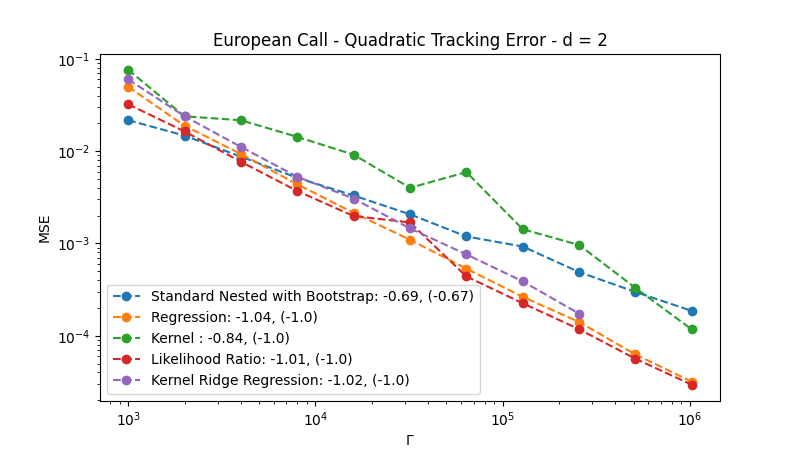
\includegraphics[width=0.9\textwidth]{../project1/figures/figure2a.png}
\end{figure}

\begin{itemize}
    \item Standard, KRR, and likelihood ratio procedures are dimension-independent
    \item Kernel smoothing and regression show sensitivity to dimension, but in different ways
\end{itemize}

\note{Previously, we worked on the asymptotic convergence rates of different nested simulation procedures. \\}
\note{In practice, the total simulation budget is finite.}
\note{When the budget is finite, the theoretical convergence rate may not be the only thing we should consider. \\}
\note{This figure shows the performance of all 5 procedures in their estimation of the quadratic tracking error for the portfolio of European call options.}
\note{It is a log-log plot of the MSE of the estimator versus the total simulation budget $\Gamma$.}
\note{For each procedure, we run 1000 macro replications of Monte Carlo simulations with different total simulation budgets. \\}
\note{For each data point on the plot, 1000 independent replications of the procedure are used to estimate the MSE. \\}
\note{The slopes of the lines estimates the empirical convergence rates of the procedures. \\}
\note{In the legend records the slopes of the lines and the corresponding asymptotic convergence rates of the procedures. \\}
\note{In the most basic case, most procedures have their empirical convergence rates match their asymptotic convergence rates. \\}
\note{However, as we will see after, this is not the case for all experiments. }

\end{frame}


\begin{frame}{Sensitivity to Asset Dimension}

    \begin{figure}
        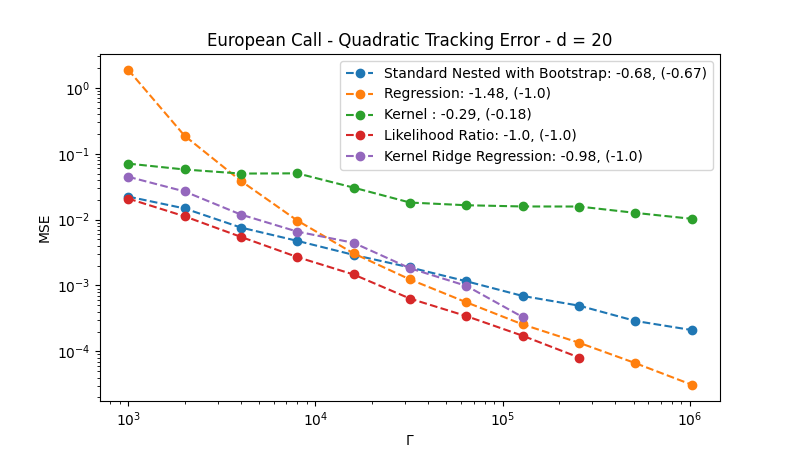
\includegraphics[width=0.9\textwidth]{../project1/figures/figure2b.png}
    \end{figure}
    
    \begin{itemize}
        \item Regression and kernel converge faster than their asymptotic rates
        \item Results of other experiments are in the thesis (Figure 2.3 - Figure 2.11)
    \end{itemize}

\note{This figure shows the same experiment as the previous figure, but we further increase the asset dimension to 20. \\}
\note{The standard procedure is not affected by the asset dimension. \\}
\note{The kernel smoothing procedure actually converges faster than what its asymptotic convergence rate suggests. \\}
\note{The regression-based procedure is the only procedure that actually converges faster when the asset dimension is high. We will do a deeper dive into it in the following experiment. \\}
\note{It is also worth noting that the likelihood ratio and KRR procedures are dimension-independent. \\}
\note{While it is not shown in their empirical rate, due to their additional cost of pooling inner replications, we are not able to run these procedures when $\Gamma$ is large. \\}
\note{In the thesis, we provide a detailed analysis of the sensitivity for all 5 procedures with more than 500 experiments. }

\end{frame}

% \begin{frame}{Fast Convergence of Regression-based Procedure}

% \begin{figure}
%     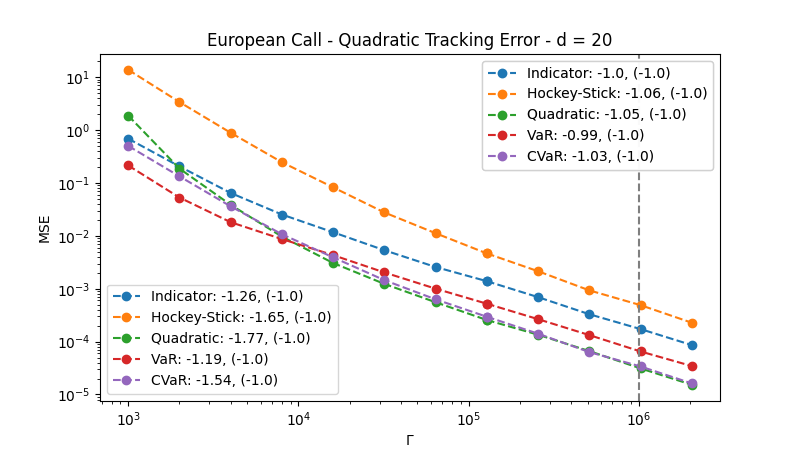
\includegraphics[width=\textwidth]{../project1/figures/figure3.png}
% \end{figure}

% \begin{itemize}
%     \item Higher initial convergence rate
%     \item Stabilizes to match asymptotic rate at higher budgets
%     \item Consistent across different asset dimensions
% \end{itemize}

% \note{To investigate the regression-based procedure, we further increase the total simulation budget $\Gamma$. \\}
% \note{The figure shows the performance of the regression-based procedure in the estimation of the quadratic tracking error for the portfolio of European call options. \\}
% \note{We separate different values of $\Gamma$ into two different parts. \\}
% \note{The first part is when $\Gamma$ is small. \\}
% \note{The second part is when $\Gamma$ is large. \\}
% \note{The first part is when the regression-based procedure has a higher convergence rate than its asymptotic convergence rate. \\}
% \note{The second part is when the regression-based procedure stabilizes and matches its asymptotic convergence rate. \\}
% \note{In our experiments, we find that the regression-based procedure is very poor when $\Gamma$ is small. \\}
% \note{It means that when we don't have enough data points, the regression-based procedure is particularly bad. \\}
% \note{As we increase the total simulation budget $\Gamma$, the regression-based procedure improves fast, and eventually matches the asymptotic convergence rate. \\}

% \end{frame}

% \begin{frame}{Sensitivity to Option Type}

% \begin{figure}
%     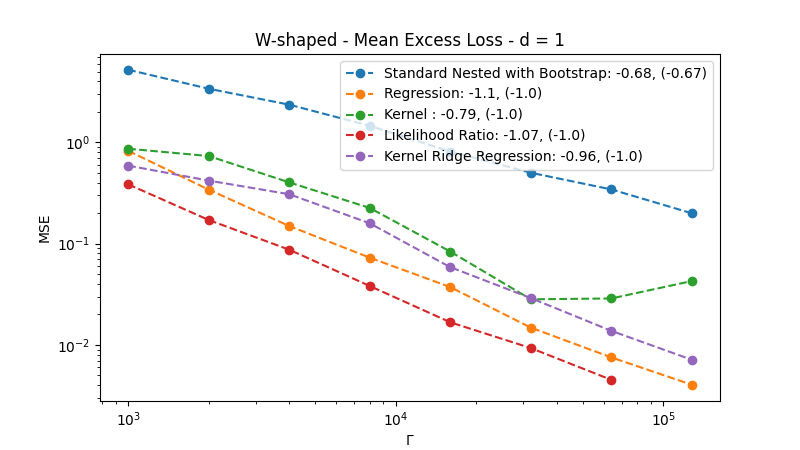
\includegraphics[width=\textwidth]{../project1/figures/figure7b.png}
% \end{figure}

% \begin{itemize}
%     \item Similar convergence patterns across different option types
%     \item Regression and kernel smoothing show higher empirical rates for barrier options
% \end{itemize}

% \note{This figure shows the performance of the procedures for a portfolio of 3 barrier options with a W-shaped payoff. \\}
% \note{This example is found in the regression-based procedure paper by broadie. It presents a case of complex payoffs for single asset dimension. \\}
% \note{Most procedures are not sensitive to the option type. \\}
% \note{The reason for kernel smoothing's MSE to increase at the right end of the plot is due to error in cross-validation of its bandwidth parameter. \\}
% \note{Due to the additional cost of cross-validation, we are not able to run it for every macro replication when the kernel smoothing procedure when $\Gamma$ is large. \\}
% \note{Instead, we use the same bandwidth parameter for all macro replications. \\}
% \note{A detailed explanation of this phenomenon is provided in the thesis. \\ }
% \note{We conducted a numerical experiment to show that the kernel smoothing procedure has sensitive cross-validation.}

% \end{frame}

% \begin{frame}{Sensitivity to Risk Measure}

%     \begin{figure}
%         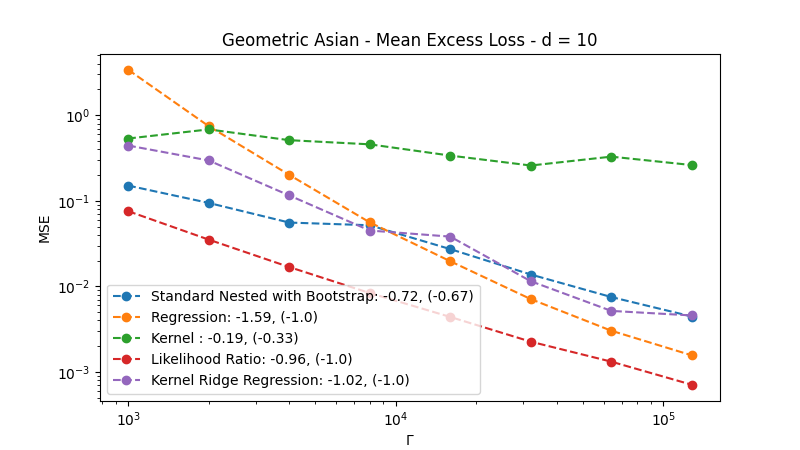
\includegraphics[width=\textwidth]{../project1/figures/figure8a.png}
%     \end{figure}
    
%     \begin{itemize}
%         \item Convergence behavior consistent across different risk measures
%     \end{itemize}
    
% \note{This figure shows the performance of the procedures for estimating the mean excess loss for a portfolio of 10 geometric Asian options on 10 underlying assets. \\}
% \note{The mean excess loss is a risk measure that involves the tail of the distribution of the portfolio loss. \\}
% \note{Most procedures are consistent across different risk measures. \\}
% \note{The kernel smoothing procedure is the only procedure that is sensitive to the risk measure. }

% \end{frame}

% \begin{frame}{Sensitivity to VaR/CVaR Level}

%     \begin{figure}
%         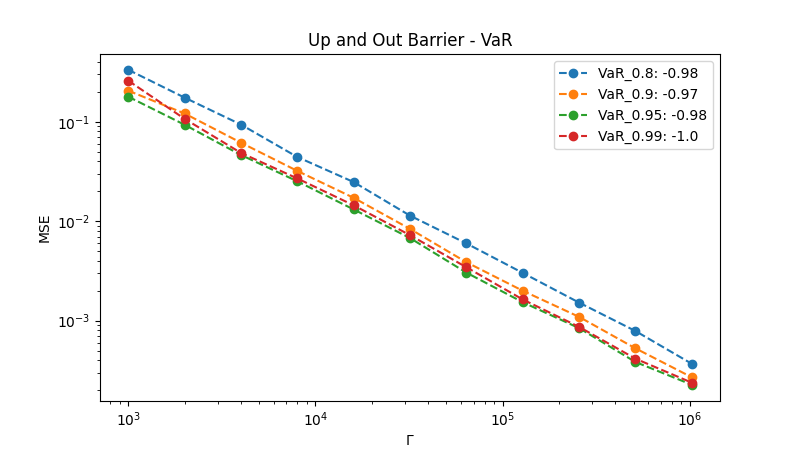
\includegraphics[width=\textwidth]{../project1/figures/figure9a.png}
%     \end{figure}
    
%     \begin{itemize}
%         \item Regression-based method not sensitive to VaR/CVaR level
%         \item Consistent performance across different levels
%     \end{itemize}
    
%     \note{From our experiments, we find that the regression procedure is cheap to implement, and its performance is consistent across different experiments. \\}
%     \note{We shift our focus to the sentivity of regression-based procedure. First, we test its sensitivity to the VaR/CVaR level. \\}
%     \note{This figure shows the performance of the regression-based procedure for different VaR/CVaR levels. \\}
%     \note{The regression-based procedure is not sensitive to the VaR/CVaR level. \\}
    
% \end{frame}
    
% \begin{frame}{Sensitivity to Asset Model}
    
%     \begin{figure}
%         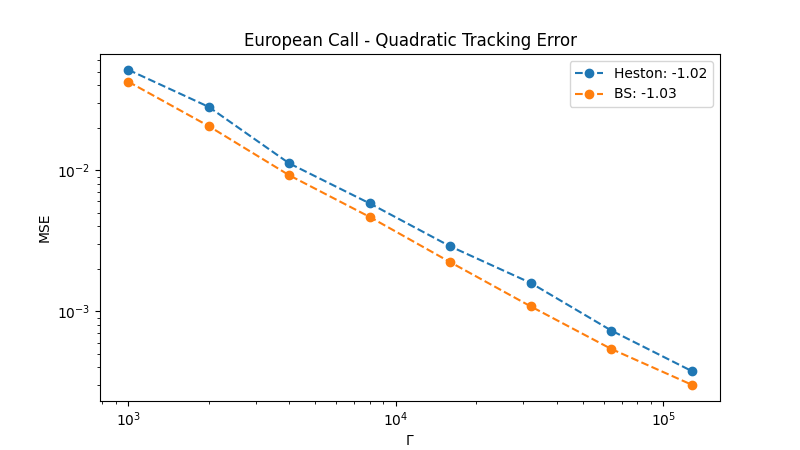
\includegraphics[width=\textwidth]{../project1/figures/figure10a.png}
%     \end{figure}
    
%     \begin{itemize}
%         \item Regression-based method insensitive to asset model (GBM vs. Heston)
%         \item Consistent performance across different asset models
%     \end{itemize}
    
%     \note{We further test the sensitivity of the regression-based procedure to the asset model. \\}
%     \note{This figure shows the performance of the regression-based procedure for different asset models. \\}
%     \note{The regression-based procedure is insensitive to the asset model. \\}
    
% \end{frame}
    
% \begin{frame}{Computational Complexity}
    
%     There are \textbf{computational costs} associated with pooling inner replications.

%     \begin{itemize}
%         \item Standard procedure: cost of estimating the optimal $M$ and $N$
%         \item Regression: most efficient among metamodel-based procedures
%         \item Kernel smoothing: costly distance calculations and cross-validation
%         \item Likelihood ratio: No training, but costly weight calculations
%         \item KRR: even more expensive than kernel smoothing
%     \end{itemize}

% \note{We have mentioned the cost of pooling inner replications multiple times. \\}
% \note{We now provide a detailed analysis of the computational complexity of different procedures. \\}
% \note{The standard procedure cannot be run without estimating the optimal $M$ and $N$. \\}
% \note{The regression procedure is the most efficient among metamodel-based procedures. \\}
% \note{The kernel smoothing procedure is costly due to the distance calculations and cross-validation. \\}
% \note{The likelihood ratio procedure does not require training, but the likelihood ratio weight calculations are costly. \\}
% \note{The KRR procedure is even more expensive than the kernel smoothing procedure due to the additional cost of the additional steps of ridge regression after the distance calculations. It also has more parameters to cross-validate. \\}


% \end{frame}

\begin{frame}{Additional Computational Costs}

    \begin{figure}
        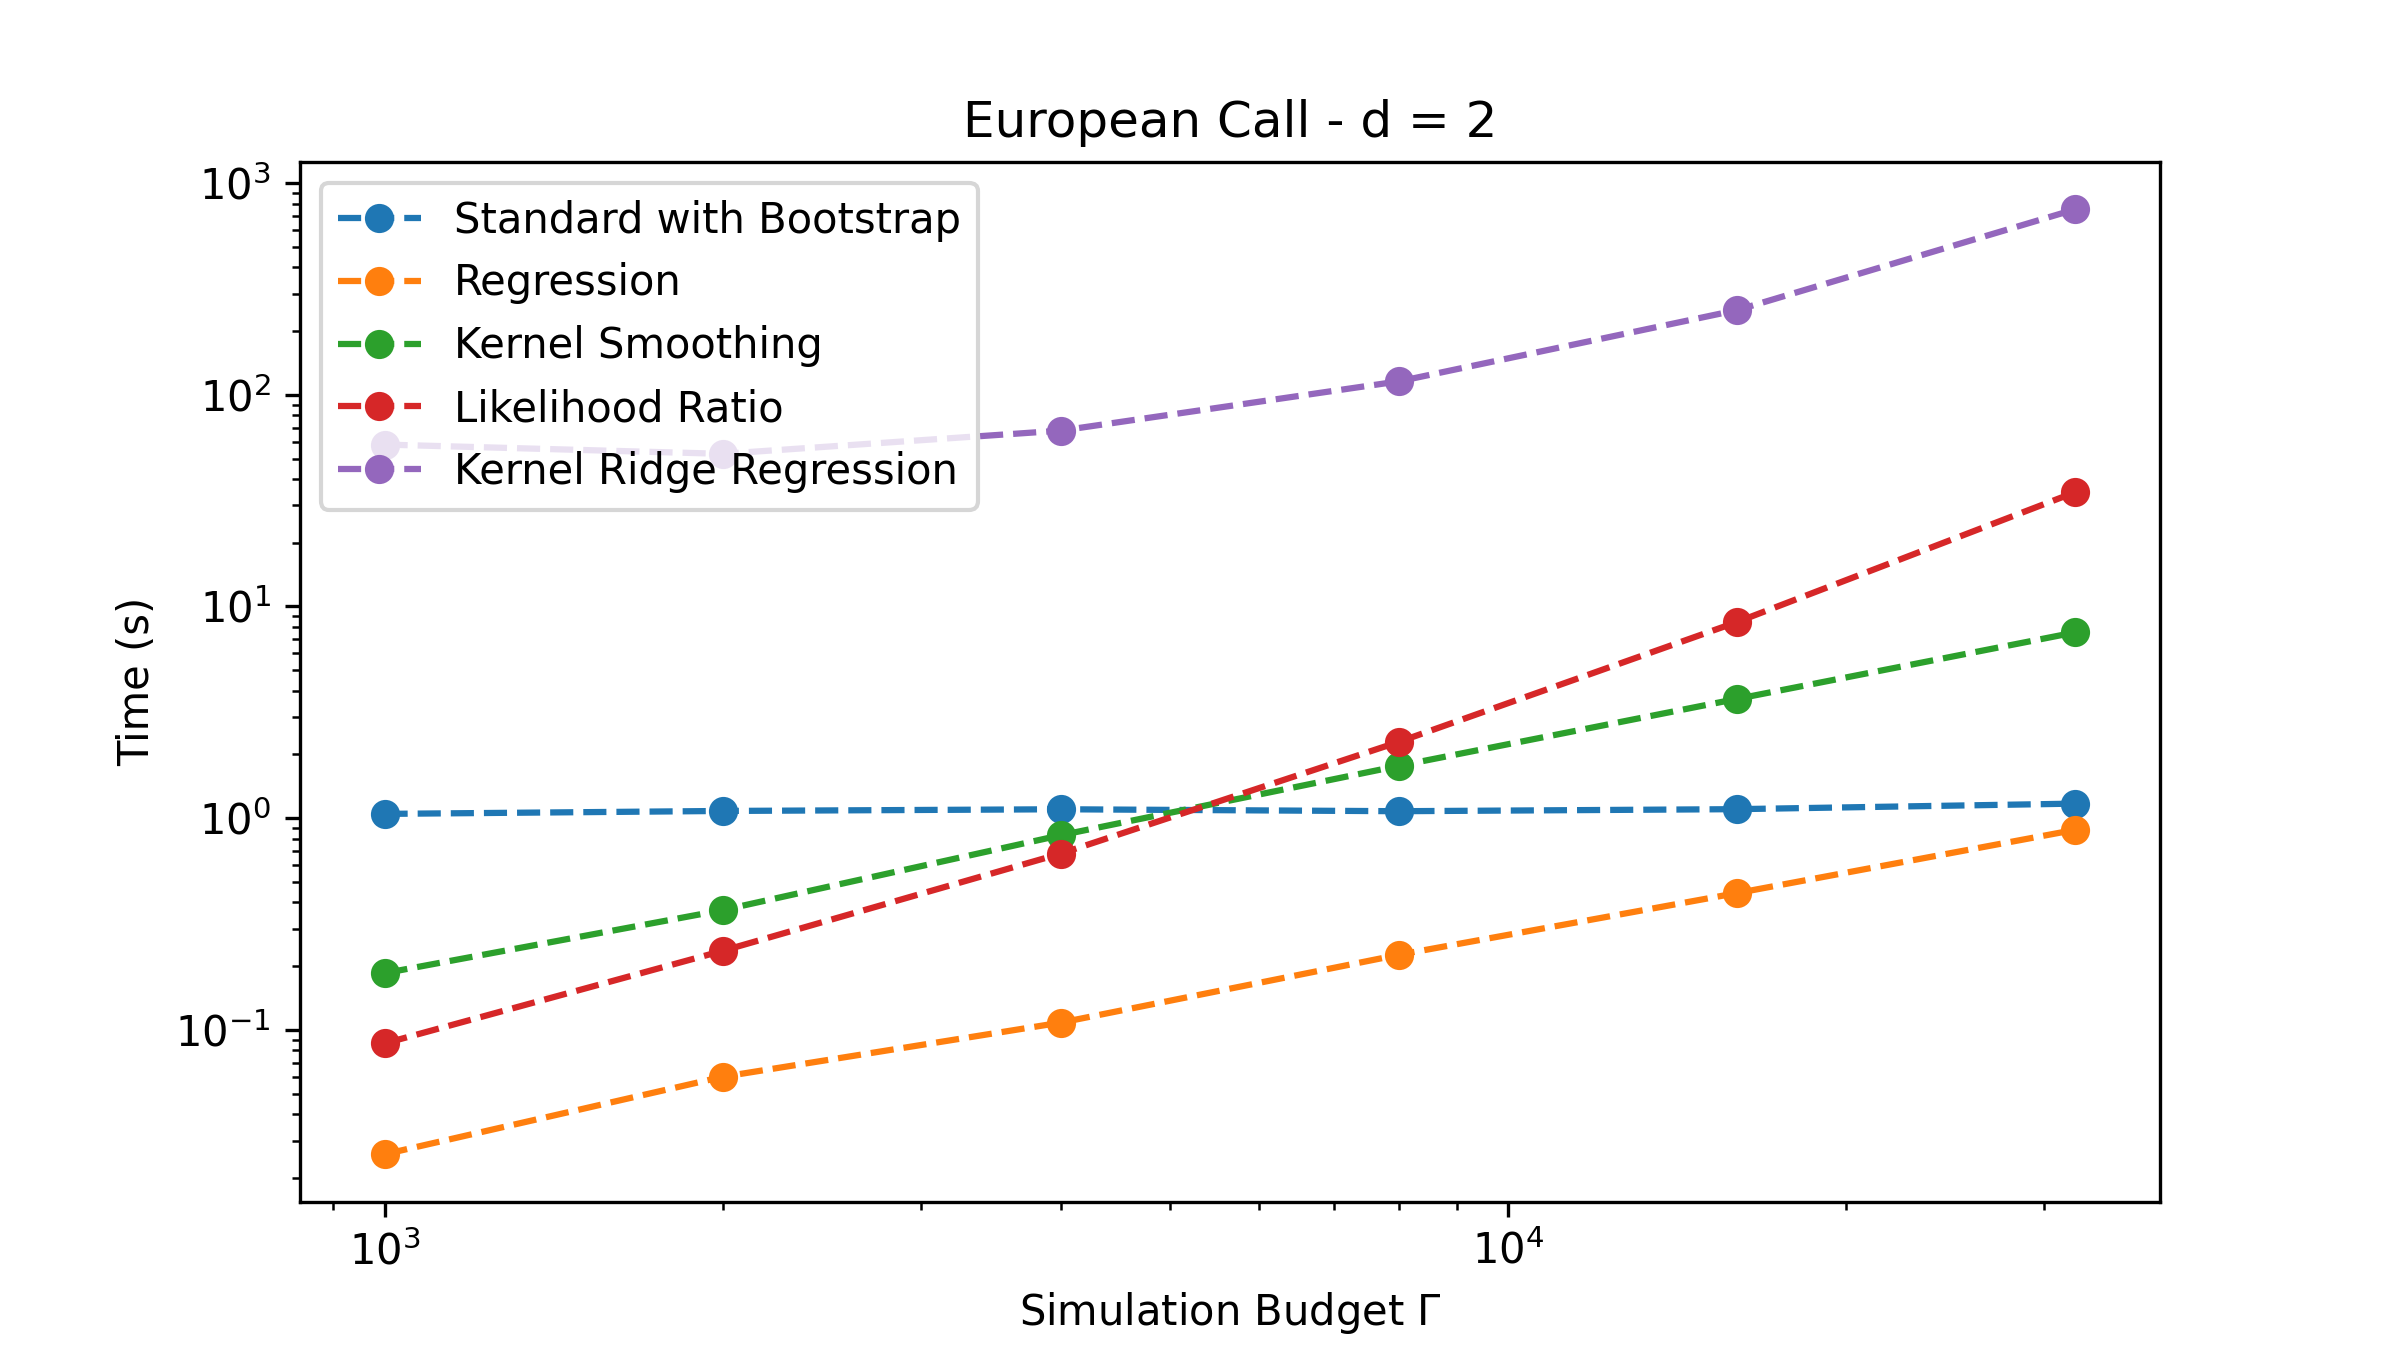
\includegraphics[width=\textwidth]{./time_comparison.png}
        \caption{Additional computation time for different procedures}
    \end{figure}

    \note{This figure shows the additional computation time for different procedures. \\}
    \note{It includes the time for training, validation, and everything else. \\}
    \note{The total computation time of the standard procedure does not increase fast with $\Gamma$. \\}
    \note{It is because the computation time of estimating the optimal $M$ and $N$ does not increase for larger $\Gamma$. \\}
    \note{Regression is the most efficient among metamodel-based procedures. \\}
    \note{The likelihood ratio and KRR are more expensive due to their additional costs. \\}
    \note{The likelihood ratio weight calculations increase quadratically with $\Gamma$. \\}
    \note{For KRR, the cost of cross-validation is too high. \\}
    \note{In the thesis includes a detailed analysis of the computational complexity of different procedures in terms of $\Gamma$.}

\end{frame}

% \begin{frame}{Cost of Hyperparameter Tuning}

%     \begin{figure}
%         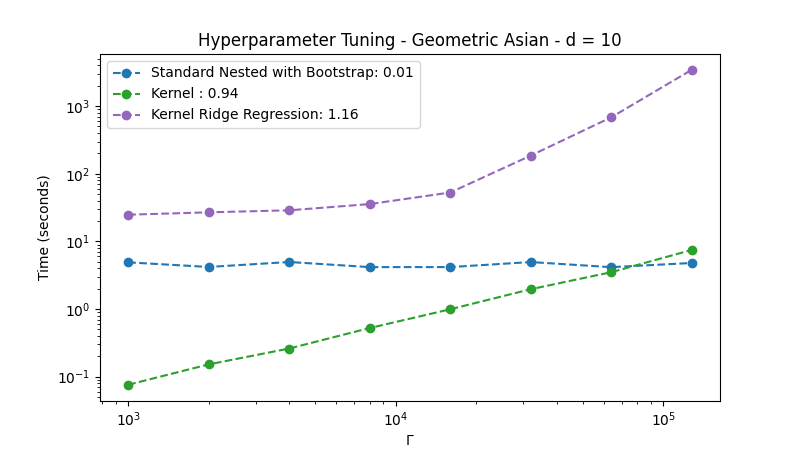
\includegraphics[width=\textwidth]{../project1/figures/figure12a.png}
%         \caption{Cost of hyperparameter tuning for different procedures}
%     \end{figure}

%     \note{We separate the additional computational cost into two parts: the cost of hyperparameter tuning and the cost of model fitting and validation. \\}
%     \note{The cost of hyperparameter tuning is the cost of running the cross-validation for the kernel smoothing procedure and KRR procedure. \\}
%     \note{$M$ and $N$ are hyperparameters for the standard procedure, so we also include the cost of estimating the optimal $M$ and $N$ in the figure. \\}
%     \note{From the figure, we can see that the cost of hyperparameter tuning contributes quite a lot to the total computation time. }
% \end{frame}

% \begin{frame}{Cost of Model Fitting and Prediction}

%     \begin{figure}
%         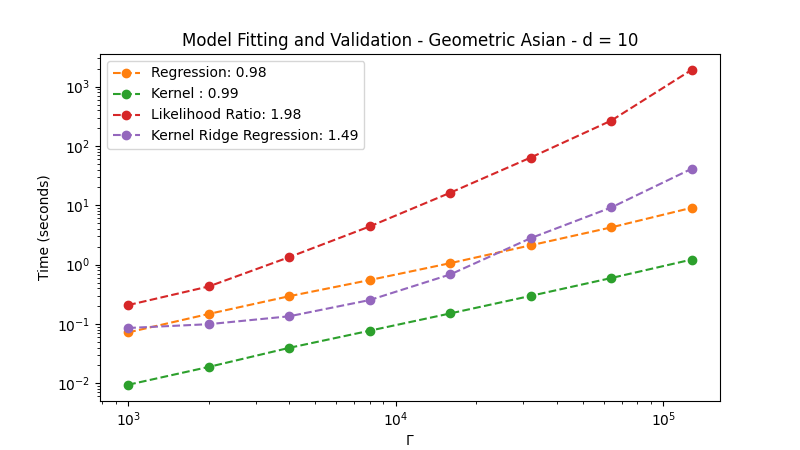
\includegraphics[width=\textwidth]{../project1/figures/figure12b.png}
%         \caption{Cost of model fitting and prediction for different procedures}
%     \end{figure}

%     \note{The cost of model fitting and prediction is the cost of fitting and using the metamodel. \\}
%     \note{We include the likelihood ratio procedure because using the likelihood ratio weights is similar to making predictions with a metamodel with fixed parameters. \\}
%     \note{We show that the regression-based and kernel-based procedures are very efficient in terms of model fitting and prediction. \\}
%     \note{Comparing the performance and the associated computational cost of different procedures, we find that the regression-based procedure is most cost-effective. \\}

% \end{frame}

\begin{frame}{Conclusion}
    Regression-based nested simulation procedure:
    \begin{itemize}
        \item Most robust and stable for limited budgets
        \item Efficient to implement
        \item Fast empirical convergence for option portfolios
    \end{itemize}

    \vspace{10pt}

    For high-dimensional or complex payoffs:
    \begin{itemize}
        \item Difficult to find a good regression basis
        \item Neural network-based procedures may be more suitable
    \end{itemize}

    \vspace{10pt}

    Next project: examining performance of metamodel-based simulation procedures for variable annuities

    \note{In our numerical experiemenct, we have shown that the regression-based procedure is the most cost-effective among all the procedures. \\}
    \note{It is robust and efficient to implement for limited budget sizes, and has fast empirical convergence for option portfolios. \\}
    \note{However, the regression-based procedure is not suitable for extremely high-dimensional risk factors or complex payoffs. \\}
    \note{The first reason is that it is hard to find a good regression basis for high-dimensional risk factors. It will involve a lot of feature engineering and expert knowledge. \\}
    \note{The second reason is that the regression-based procedure is not able to capture the nonlinearity in the payoff. \\}
    \note{In the next project, we will examine the performance of metamodel-based simulation procedures for variable annuities. \\}
    \note{This is where a neural network-based procedure can be more suitable as a form of automated feature engineering. }

\end{frame}

\section[Using DNNs for Nested Simulation]{Cutting Through the Noise: Using Deep Neural Network Metamodels for High-Dimensional Nested Simulation}

% \begin{frame}{From Options to Variable Annuities}

%     Variable annuities (VAs) poses a challenge for nested simulation due to its \textbf{high-dimensional} and \textbf{complex payoff structure}.

%     \vspace{10pt}

%     \begin{figure}[H]
%             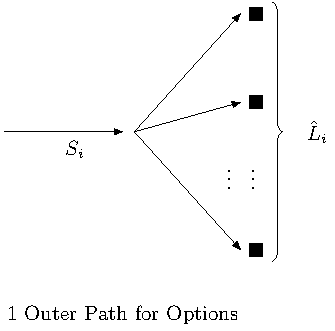
\includegraphics[width=0.33\textwidth]{./tikz/illustration_spns.pdf}
%             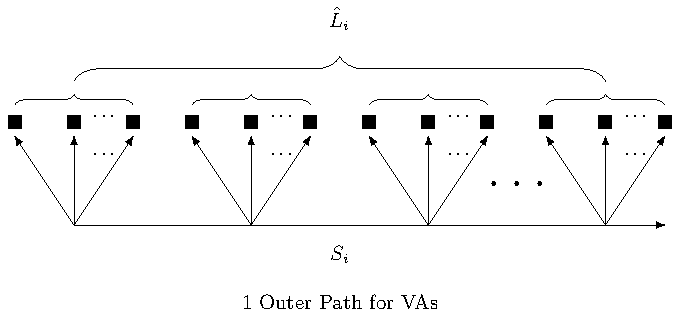
\includegraphics[width=0.62\textwidth]{./tikz/illustration_mpns.pdf}
% 	\end{figure}

%     \vspace{10pt}

%     \begin{itemize}
%         \item Need to reconstruct a metamodeling-based nested simulation procedure
%     \end{itemize}

%     \note{Variable annuities poses a challenge for nested simulation due to its high-dimensional and complex payoff structure. \\}
%     \note{A regression-based procedure is not suitable. We need to reconstruct a metamodeling-based nested simulation procedure for VAs. \\}
%     \note{On the left is the illustration of our previous nested simulation procedure for options. \\}
%     \note{On the right is the illustration of the nested simulation procedure for VAs. \\}
%     \note{The main difference is that the payoff of VAs, when dynamic hedging is present, is a function of the entire path of the underlying asset. \\}
%     \note{In terms of metamodeling with machine learning, the feature is a time series of the underlying asset, and the label is the payoff of the VA with dynamic hedging. \\}

% \end{frame}

\begin{frame}{Nested Simulation for Risk Management of VAs}

    \begin{figure}[c]
        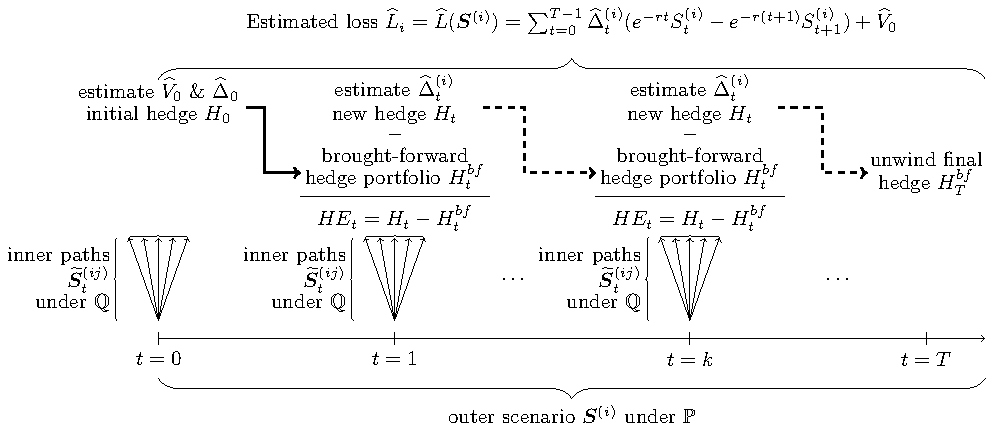
\includegraphics[width=\textwidth]{../project2/figures/sns.pdf}
        \caption{Illustration of nested simulation that estimates the P\&L for one outer scenario}
    \end{figure}

    \note{The main difference of the standard nested simulation of VAs can be explained by this illustration. \\}
    \note{This is how the P\&L is estimated for one outer scenario. \\}
    \note{It starts at $t=0$ with a simulation to estimate the initial value of the VA contract and the initial hedge. Here we are using delta-hedging. \\}
    \note{This hedge gets carried forward and updated at each time period with another simulation. \\}
    \note{The P\&L is then estimated by adding up the hedging error at each time period to the initial value of the VA contract. \\}
    \note{All the simulation mentioned is a single set of inner simulations for one outer scenario. \\}
    \note{It is very expensive to run this standard nested simulation for VAs. \\}

\end{frame}

% \begin{frame}{Standard Nested Simulation for VAs}

% Standard nested simulation for VAs is similar to the one for options.

% \begin{itemize}
%     \item Generate $M$ outer scenarios
%     \item For each outer scenario,
%     \begin{itemize}
%         \item Perform $N$ inner simulations
%         \item Estimate hedging loss $L_i$ with $\hat{L}_i$
%     \end{itemize}
%     \item Use estimated losses to calculate tail risk measures (e.g., $95\%$-CVaR)
% \end{itemize}

% \vspace{10pt}

% \textbf{Observations:}
% \begin{itemize}
%     \item computational budget is limited;
%     \item high-dimensional input space;
%     \item only a \textbf{small} portion of scenarios are relevant when estimating \textbf{tail} risk measures.
% \end{itemize}

% \note{The standard nested simulation for VAs is similar to the one for options. \\}
% \note{First, we generate $M$ outer scenarios. \\}
% \note{For each outer scenario, we perform $N$ inner simulations to estimate the hedging loss $L_i$ with $\hat{L}_i$. \\}
% \note{Then, we use the estimated losses to calculate tail risk measures, such as a $95\%$-CVaR. \\}
% \note{The main difference is that the payoff of VAs, when dynamic hedging is present, is a function of the entire path of the underlying asset. \\}
% \note{In terms of metamodeling with machine learning, the feature is a time series of the underlying asset, and the label is the payoff of the VA with dynamic hedging. \\}
% \note{The computational budget is limited, and the input space is high-dimensional. \\}
% \note{Only a small portion of scenarios are relevant when estimating tail risk measures. \\}
% \note{In this project, we propose a metamodel-based nested simulation procedures to concentrate the simulation on the relevant scenarios. \\}

% \end{frame}

\begin{frame}{Metamodel-based Nested Simulation}

    We use deep neural networks (DNNs) as metamodels 
    \begin{itemize}
        \item Use LSTMs for sequential data
        \item \textbf{Challenge}: lack of transparency and interpretability
    \end{itemize}

    \vspace{20pt}

    \textbf{Research Contributions:}
    \vspace{6pt}
    \begin{enumerate}
        \item Propose two generic DNN-based nested simulation procedures
        \begin{itemize}
            \item   Accurate tail scenario identification
            \item   Significant computational savings by \textbf{budget concentration}
        \end{itemize}
        \vspace{6pt}
        \item Study noise tolerance of DNNs using simulated data
        \begin{itemize}
            \item \textbf{Control noise levels} by adjusting simulation parameters
            \item Provide direct evidence on transparency and interpretability
        \end{itemize}
    \end{enumerate}

\note{After numerical experiments, we find that the deep neural network metamodels are suitable for this problem. \\}
\note{We use LSTM for the sequential data. It provides accurate tail scenario identification and significant computational savings by budget concentration. \\}
\note{However, it is not transparent and interpretable. Many researchers are working on this topic. \\}
\note{This is where we can contribute to the research. \\}
\note{By using nested simulation as a data generating process, we can study the noise tolerance of DNNs. \\}
\note{The noise level in the training labels can be controlled by adjusting the simulation parameters. \\}
\note{By examining the performance of DNNs with different noise levels, we can provide direct evidence on the transparency and interpretability of DNNs. \\}

\end{frame}

\begin{frame}{Two-Stage Metamodel-based Nested Simulation}

\begin{algorithm}[H]
    \caption{Two-Stage Metamodel-based Nested Simulation for VAs}

\begin{algorithmic}[1]
    \STATE{\textbf{Generate training data for metamodels}}
    % \begin{itemize}
    %     \item Use a fraction of the simulation budget to run the standard nested simulation procedure with $M$ outer scenarios and $N'$ inner replications.
    %     \item Construct feature-label pairs $\{(X_i, Y_{ij}) : i=1, \ldots, M, j=1, \ldots, N'\}$
    % \end{itemize}
    \STATE{\textbf{Train metamodels}}
    % \begin{itemize}
    %     \item Use the feature-label pairs to train a metamodel.
    %     \item Use the trained metamodel to make predictions for $\{X_i: i=1, \ldots, M\}$.
    %     \item Sort the predicted losses to identify a predicted tail scenario set that contains the $m$ largest predicted losses.
    % \end{itemize}
    \STATE{\textbf{Estimate $\alpha$-CVaR with extensive simulation on \textcolor{color10_5}{predicted tail scenarios}}}
    \begin{itemize}
        \item  Concentrate simulation on predicted tails
    \end{itemize}
\end{algorithmic}
\end{algorithm}

\vspace{10pt}

\textbf{Key Findings:}
\begin{itemize}
    \item   Substantial computational savings ($70\% - 85\%$ reduction)
    \item   Some DNN metamodels make \textbf{accurate loss predictions}
\end{itemize}

\note{The two-stage procedure is a two-step process that is based on the idea of budget concentration. \\}
\note{First, we generate training data for the metamodel. \\}
\note{We use a fraction of the simulation budget to run the standard nested simulation procedure with $M$ outer scenarios and $N'$ inner replications. \\}
\note{We then train a metamodel using the feature-label pairs. \\}
\note{We use the trained metamodel to make predictions for all outer scenarios. \\}
\note{We then identify the predicted tail scenario set that contains the $m$ largest predicted losses. \\}
\note{Finally, we run the standard nested simulation procedure on the predicted tail scenarios. \\}

\end{frame}


% \begin{frame}{Benefits of a Two-Stage Procedure}


% Simulation budget can be saved when:
% \begin{itemize}
%     \item the metamodel is accurate (a small $m$ includes most tail scenarios)
%     \item the metamodel can tolerate noise in training labels (a small $N'$)
% \end{itemize}

% \vspace{10pt}

% \textbf{Key findings:}
% \begin{itemize}
%     \item Substantial computational savings ($70\% - 85\%$ reduction)
%     \item Maintains accuracy comparable to standard procedure
%     \item DNN metamodels can distinguish between tail and non-tail scenarios effectively
%     \item Addresses regulatory concerns by using actual simulations for final estimates
% \end{itemize}

% \vspace{10pt}
% \textbf{Another finding:} 
% some DNN metamodels make \textbf{accurate loss predictions} for given scenarios.

% \note{The two-stage procedure can save substantial computational budget when the metamodel is accurate and can tolerate noise in training labels. \\}
% \note{By concentrating the simulation on the predicted tail scenarios, the two-stage procedure can achieve a comparable accuracy to the standard procedure while using only a fraction of the simulation budget. \\}
% \note{This approach also addresses regulatory concerns by using actual simulations for final estimates. \\}
% \note{It is also worth noting that we found some DNN metamodels that can make accurate loss predictions for given scenarios. \\}
% \note{Why don't we use these metamodels to make predictions directly? So, we propose a single-stage procedure to avoid the second stage of the two-stage procedure.}

% \end{frame}


\begin{frame}{Single-Stage Metamodel-based Nested Simulation}

    \begin{algorithm}[H]
        \caption{Single-Stage Metamodel-based Nested Simulation for VAs}
    
    \begin{algorithmic}[1]
        \STATE{\textbf{Generate training data for metamodels}}
        % \begin{itemize}
        %     \item Use a fraction of the simulation budget to run the standard nested simulation procedure with $M$ outer scenarios and $N'$ inner replications.
        %     \item Construct feature-label pairs $\{(X_i, Y_{ij}) : i=1, \ldots, M, j=1, \ldots, N'\}$
        % \end{itemize}
        \STATE{\textbf{Train metamodels}}
        % \begin{itemize}
        %     \item Use the feature-label pairs to train a metamodel.
        %     \item Use the trained metamodel to make predictions for $\{X_i: i=1, \ldots, M\}$.
        %     \item Sort the predicted losses to identify a predicted tail scenario set that contains the $m$ largest predicted losses.
        % \end{itemize}
        \STATE{\textbf{Estimate $\alpha$-CVaR with \textcolor{color10_5}{metamodel predictions}}}
        \begin{itemize}
            \item  Entirely avoids extensive simulation
        \end{itemize}
    \end{algorithmic}
    \end{algorithm}

\vspace{10pt}

\textbf{Key advantages:}
\begin{itemize}
    \item more efficient than a two-stage procedure;
    \item avoids specifying a safety margin $m$.
\end{itemize}

\note{The single-stage procedure shares the same idea of running the standard nested simulation procedure to generate training data for the metamodel. \\}
\note{After a metamodel is trained, we use it to make predictions for VA contract losses accross all outer scenarios. \\}
\note{The risk measure is estimated using the predicted losses of the metamodel. \\}
\note{It is more efficient than the two-stage procedure because it avoids the second stage of the two-stage procedure. \\}
\note{It also avoids specifying a safety margin $m$, which is a feature of the two-stage procedure that we will discuss later.}

\end{frame}

% \begin{frame}{Experiment Setting}

%     We estimate the $95\%$-CVaR of the hedging loss for a GMWB contract with 20-year maturity.

%     \vspace{10pt}

%     \textbf{Specifications:}
%     \begin{itemize}
%         \item The underlying asset follows a regime-switching geometric Brownian motion;
%         \item The contract is delta-hedged monthly (240 periods);
%         \item The true $95\%$-CVaR is estimated using 100,000 outer scenarios and 100,000 inner replications.
%         \item The metamodel is trained using 90,000 outer scenarios and 100 inner replications.
%         \item Benchmark: standard nested simulation procedure with 100,000 outer scenarios and 1,000 inner replications.
%     \end{itemize}

% \note{In our numerical experiments, we consider a GMWB contract with 20-year maturity. \\}
% \note{The underlying asset follows a regime-switching geometric Brownian motion. \\}
% \note{The contract is delta-hedged monthly (240 periods). \\}
% \note{The true $95\%$-CVaR is estimated using 100,000 outer scenarios and 100,000 inner replications. We call this the true data. \\}
% \note{The metamodel is trained using 90,000 outer scenarios and 100 inner replications, called the training data. \\}
% \note{Another 10,000 outer scenarios with 100 inner replications are used to evaluate the performance of the metamodel, called the test data. \\}
% \note{The true data is not available in practice, but it is useful for evaluating the performance of the metamodel. \\}
% \note{The difference in performance between the training data and the test data, and between the test data and the true data, provides insights into the noise tolerance of the metamodel. \\}
% \note{And it helps us to understand an important question: what does deep neural networks learn from noisy data? \\}
% \note{For our experiments, the benchmark is the standard nested simulation procedure with 100,000 outer scenarios and 1,000 inner replications. }

% \end{frame}

\begin{frame}{Experiment Setting}

    We consider the following metamodel architectures:

    \begin{table}[ht!]
        \centering
        \begin{tabular}{lcc}
            \toprule
            \textbf{Metamodel} & \textbf{Abbreviation} & \textbf{Capacity} \\
            \midrule
            Multiple Linear Regression      & MLR       & 241 \\
            Quadratic Polynomial Regression & QPR       & 481 \\
            Feedforward Neural Network      & FNN       & 35,009 \\
            Recurrent Neural Network        & RNN       & 32,021 \\
            Long Short-Term Memory          & LSTM      & 35,729 \\
            \bottomrule
        \end{tabular}
        \caption{Metamodel architectures for GMWB inner simulation model}
        \label{tab:arch}
    \end{table}

    In our experiment:
    \begin{itemize}
        \item $95\%$-CVaR of loss for a GMWB with a 240-month maturity
        \item 240-dimensional feature vector and 1-dimensional loss
    \end{itemize}

    \note{We consider the following metamodel architectures: \\}
    \note{Multiple Linear Regression, Quadratic Polynomial Regression, Feedforward Neural Network, Recurrent Neural Network, and Long Short-Term Memory Network. \\}
    \note{Capacity is defined as the number of parameters in the metamodel. \\}
    \note{Higher capacity metamodels are more flexible and expressive. \\}
    \note{Lower capacity metamodels are less likely to overfit. \\}
    \note{The deep neural network metamodels are more flexible and expressive, but they are said to be more prone to overfitting. \\}
    \note{We will see whether this is indeed the case in our experiments. \\}
    
\end{frame}



\begin{frame}{Metamodel Performance}

    \begin{figure}[H]
        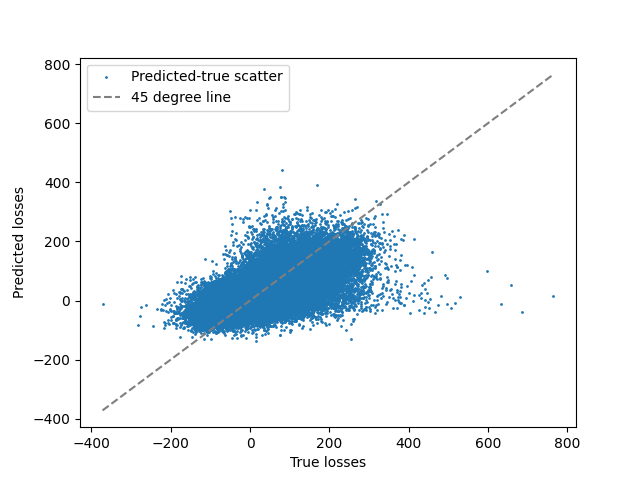
\includegraphics[width=0.48\textwidth]{../project2/figures/qqPlots/qprLN.png}
        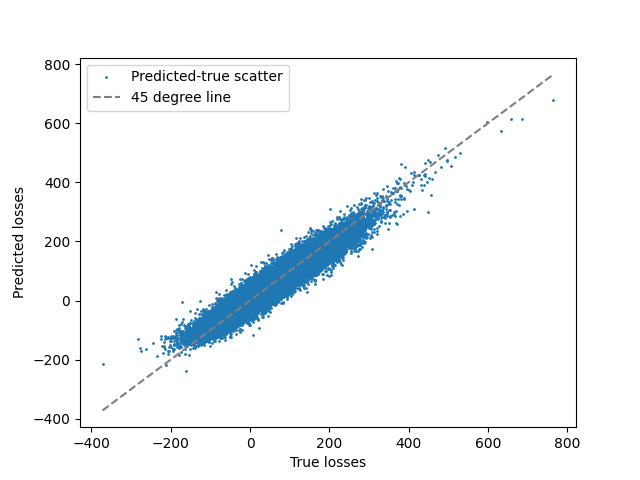
\includegraphics[width=0.48\textwidth]{../project2/figures/qqPlots/lstmLoCapLN.png}
        \caption{QQ plots between true and predicted loss labels for QPR and LSTM metamodels}
    \end{figure}

    \begin{itemize}
        \item   QPR make \textbf{inaccurate} loss predictions
        \item   DNN metamodels are more flexible.
    \end{itemize}

    \note{We first take a look at their performance with QQ plots. \\}
    \note{On the left is the QQ plot between the true loss labels and the predicted loss labels for QPR, and on the right is the QQ plot for LSTM. \\}
    \note{Feature engineering for QPR is hardly feasible for our 240-dimensional $X$. Its poor performance is expected. \\}
    \note{DNN metamodels are more flexible, and they can make more accurate loss predictions. \\}

\end{frame}

% \begin{frame}{Deep Neural Network Metamodels}

%     \begin{figure}[H]
%         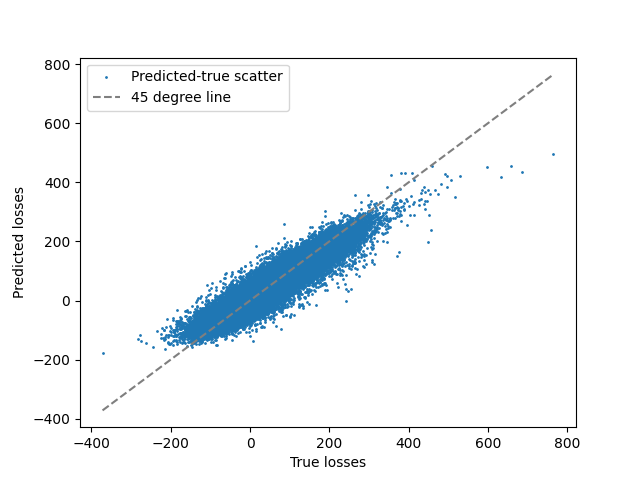
\includegraphics[width=0.48\textwidth]{../project2/figures/qqPlots/fnnLN.png}
%         \caption{QQ plots between true and predicted loss labelsfor FNN and LSTM metamodels}
%     \end{figure}

%     \begin{itemize}
%         \item   DNN metamodels are more flexible.
%         \item   Time series features prefer LSTM over FNN.
%         \item   Network architecture serves as regularization.
%     \end{itemize}

%     \note{We then consider the deep neural network metamodels. \\}
%     \note{On the left is the QQ plot between the true loss labels and the predicted loss labels for FNN, and on the right is the QQ plot for LSTM. \\}
%     \note{DNN metamodels are more flexible. \\}
%     \note{We find that our time series outer scenarios prefer a LSTM metamodel over FNN. \\}
%     \note{Network architecture is thought to serve as prior knowledge that regularizes DNNs. \\}
%     \note{It decides how the individual neurons are connected to each other. \\}
%     \note{For example, FNN is a fully-connected network, meaning that we don't impose any structure on the connections between neurons. \\}
%     \note{In contrast, LSTM has a recurrent structure, meaning that the connections between neurons are time-dependent. \\}

% \end{frame}


\begin{frame}{Research Questions}

    \begin{itemize}
        \item What do DNNs learn from noisy data?
        \item How well do DNNs learn from noisy data?
    \end{itemize}

    \begin{figure}[H]
        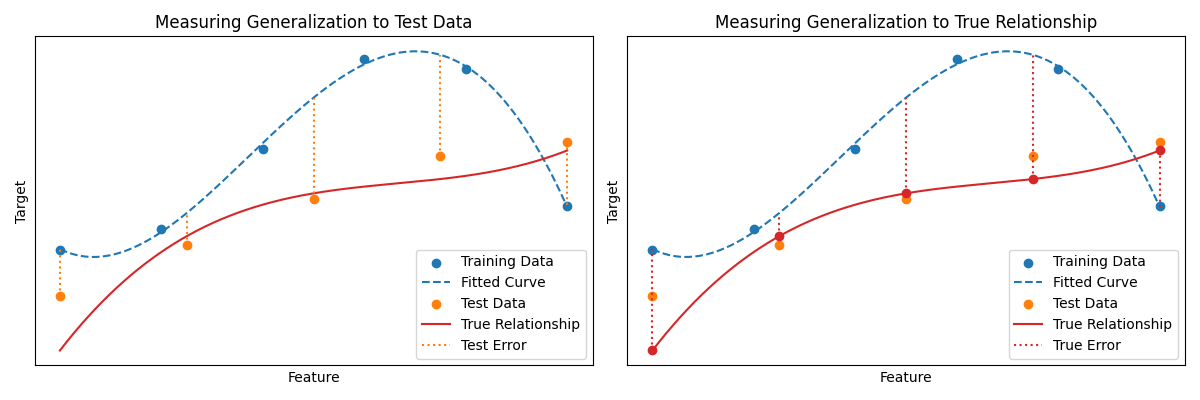
\includegraphics[width=\textwidth]{../project2/figures/datasets.png}
    \end{figure}

    Three datasets are considered:
    \begin{itemize}
        \item   \textcolor{color10_2}{Training}: 90,000 scenarios (100 inner replications).
        \item   \textcolor{color10_3}{Test}: 10,000 scenarios (100 inner replications).
        \item   \textcolor{color10_5}{True}: 100,000 scenarios (100,000 inner replications).
    \end{itemize}


\note{To further clarify our research questions, we consider the following scenario: \\}
\note{We have a noisy training data and a noisy test data. \\}
\note{We want to know what the metamodel learns from the noisy data. \\}
\note{We also want to know how well the metamodel can make accurate loss predictions for given scenarios. \\}
\note{In a simulation experiment, we can control the noise level in the training data and the test data. \\}
\note{We also have access to the true feature-label relationship when we increase the number of replications. \\}
\note{We can use this true feature-label relationship to evaluate the performance of deep neural networks, which is usually not possible in practice. }

\end{frame}

\begin{frame}{Metamodel Performance on Different Datasets}

    \begin{table}[ht!]
        \centering
        \small
        \begin{tabular}{lccc}
        \toprule
        \textbf{Metamodel} & \textcolor{color10_2}{\textbf{Training error}} & \textcolor{color10_3}{\textbf{Test error}} & \textcolor{color10_5}{\textbf{True error}}\\
        \midrule
        MLR & $\textcolor{color10_2}{0.706}$ $(\pm 8.3\times 10^{-4})$ & $\textcolor{color10_3}{0.713}$ $(\pm 2.7 \times 10^{-2})$ & $\textcolor{color10_5}{0.706}$ $(\pm 3.4 \times 10^{-4})$ \\
        QPR & $\textcolor{color10_2}{0.543}$ $(\pm 8.3\times 10^{-4})$ & $\textcolor{color10_3}{0.554}$ $(\pm 2.7 \times 10^{-2})$ & $\textcolor{color10_5}{0.544}$ $(\pm 4.1 \times 10^{-4})$ \\
        FNN & $\textcolor{color10_2}{0.129}$ $(\pm 6.0\times 10^{-3})$ & $\textcolor{color10_3}{0.240}$ $(\pm 9.8 \times 10^{-3})$ & $\textcolor{color10_5}{0.132}$ $(\pm 5.8 \times 10^{-3})$ \\
        RNN & $\textcolor{color10_2}{0.132}$ $(\pm 7.5\times 10^{-3})$ & $\textcolor{color10_3}{0.137}$ $(\pm 7.6 \times 10^{-3})$ & $\textcolor{color10_5}{0.119}$ $(\pm 7.5 \times 10^{-3})$ \\
        LSTM & \textbf{$\textcolor{color10_2}{0.075}$} $(\pm 4.5\times 10^{-3})$ & \textbf{$\textcolor{color10_3}{0.079}$} $(\pm 5.4 \times 10^{-3})$ & \textbf{$\textcolor{color10_5}{0.063}$} $(\pm 4.4 \times 10^{-3})$ \\
        RNN$^*$\footnotemark & $\textcolor{color10_2}{0.109}$ $(\pm 5.2\times 10^{-3})$ & $\textcolor{color10_3}{0.128}$ $(\pm 5.2 \times 10^{-3})$ & $\textcolor{color10_5}{0.109}$ $(\pm 5.2 \times 10^{-3})$ \\
        \bottomrule
        \end{tabular}
        \caption{Average MSEs and 95\% confidence bands of metamodels for GMWB.}
        \label{tab:gmwb_arch}
    \end{table}

    \footnotetext{This row summarizes the results of the well-trained RNNs.}

    \begin{itemize}
        \item   RNN-based metamodels have lower true errors than their training errors.
        \item   DNN metamodels with suitable architectures \textbf{cut through the noise} in training labels.
    \end{itemize}

    \note{This table summarizes the results of our experiments. \\}
    \note{It is the most interesting finding that DNN metamodels with suitable architectures can \textbf{cut through the noise} in training labels. \\}
    \note{The average MSEs of metamodels on the training, test, and true data are reported in the three columns, respectively. \\}
    \note{Note that the training and test labels are noisy. The simulation noise is what makes them noisy, which is less present in the true data. \\}
    \note{First, we note that DNN metamodels has lower training errors than the traditional regression metamodels. \\}
    \note{This is expected because DNNs are more flexible and expressive than traditional regression metamodels. \\}
    \note{What is more interesting is the comparison between the test and true errors. \\}
    \note{We find that the true errors of RNN-based metamodels are lower than their test errors. \\}
    \note{This suggests that the RNN and LSTM metamodels can learn the true feature-label relationship. \\}
    \note{When we take another look at the table, we find that for LSTM, its true error is even lower than its training error. \\}
    \note{This is another evidence that LSTM metamodels are able to cut through the noise in training labels and fit to the true relationship. \\}
    \note{RNN metamodels suffer from the vanishing gradient problem. This is why we make separate rows for well-trained RNNs and poorly-trained RNNs. }

\end{frame}

% \begin{frame}{Issues with Crude RNNs}

%     \begin{figure}[H]
%         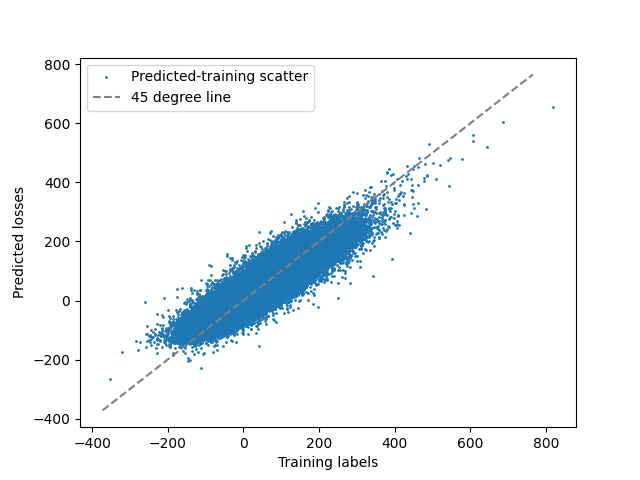
\includegraphics[width=0.48\textwidth]{../project2/figures/qqPlots/rnnGood_training.png}
%         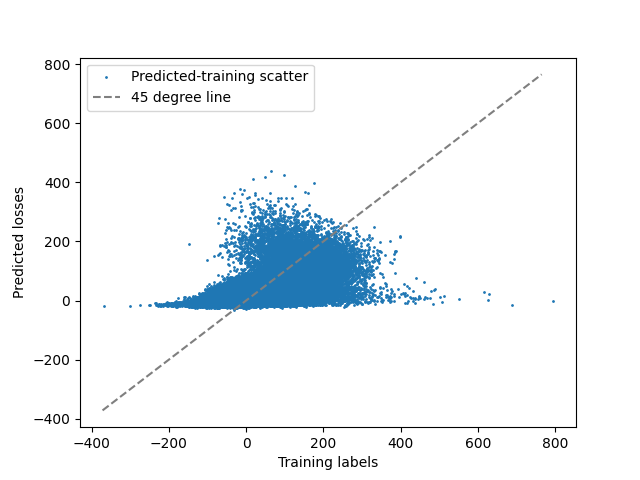
\includegraphics[width=0.48\textwidth]{../project2/figures/qqPlots/rnnBad_training.png}
%         \caption{QQ plots between training and predicted loss labels for RNN metamodels}
%     \end{figure}

%     \begin{itemize}
%         \item   RNN metamodels suffers from \textbf{vanishing gradient problem}.
%         \item   Ease of training (reliability) is a critical factor when choosing a DNN metamodel.
%     \end{itemize}

%     \note{The QQ plots on the left show the relationship between the training and predicted loss labels for a well-trained RNN, and on the right is a poorly-trained RNN. \\}
%     \note{We find that the well-trained RNN has a better relationship between the training and predicted loss labels. \\}
%     \note{However, the poorly-trained RNN suffers from the vanishing gradient problem. \\}
%     \note{It is unable to continue learning from the training data. \\}
%     \note{During our training some RNNs suffer from gradient explosion. \\}
%     \note{The training process is highly unstable. \\}
%     \note{This issue can be mitigated by using gradient clipping and other techniques. However, it can not be completely avoided. \\}
%     \note{Therefore, we recommend using LSTM metamodels over RNN metamodels. \\}

% \end{frame}

\begin{frame}{Safety Margin}


    Consider estimating the $95\%$ CVaR with 100,000 outer scenarios.
    \begin{figure}
        \centering
        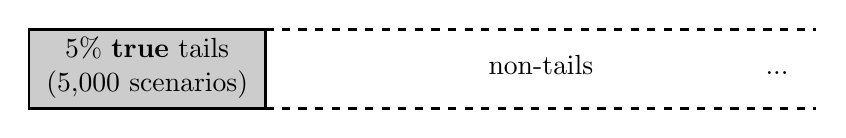
\begin{tikzpicture}[scale=1]
            % Make the height of the solid rectangle half.
            \draw[line width=1pt, fill=gray, fill opacity=0.40] (0,0) rectangle (3,1); 
            % Adjust node positions for the new height.
            \node[above] at (1.5, 0.5) {5\% \textbf{true} tails}; 
            \node[above] at (1.5, 0) {(5,000 scenarios)};
            % Adjust the dashed lines for the new height.
            \draw[dashed, line width=1pt] (3,0) -- (10,0); 
            \node[above] at (6.5, 0.3) {non-tails};
            \draw[dashed, line width=1pt] (3,1) -- (10,1); 
            \node[above] at (9.5, 0.3) {...};
        \end{tikzpicture}
    \end{figure}
    \begin{figure}
        \centering
        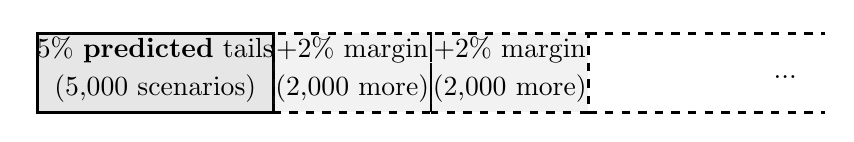
\begin{tikzpicture}[scale=1]
            % Make the height of the solid rectangle half.
            \draw[line width=1pt, fill=gray, fill opacity=0.20] (0,0) rectangle (3,1);
            % Adjust node positions for the new height.
            \node[above] at (1.5, 0.5) {5\% \textbf{predicted} tails};
            \node[above] at (1.5, 0) {(5,000 scenarios)};
            % Adjust the dashed boxes for the new height.
            \draw[dashed, line width=1pt, fill=gray, fill opacity=0.10] (3,0) rectangle (5,1);
            \node[above] at (4, 0.5) {+2\% margin};
            \node[above] at (4, 0) {(2,000 more)};
            \draw[dashed, line width=1pt, fill=gray, fill opacity=0.10] (5,0) rectangle (7,1);
            \node[above] at (6, 0.5) {+2\% margin};
            \node[above] at (6, 0) {(2,000 more)};
            % Adjust the dashed lines for the new height.
            \draw[dashed, line width=1pt] (7,0) -- (10,0);
            \draw[dashed, line width=1pt] (7,1) -- (10,1);
            \node[above] at (9.5, 0.3) {...};
        \end{tikzpicture}
        \caption{Illustration: a safety margin of $4\%$ ($m = 9000$)}
    \end{figure}
    
    \vspace{10pt}
    \textbf{Trade-off between accuracy and efficiency}
    \begin{itemize}
        \item   Lower margin: not enough tail identified
        \item   Higher margin: more budget spent on extensive simulation
    \end{itemize}

    \note{For a two-stage procedure, we need to choose a safety margin $m$ to identify the tail scenarios. \\}
    \note{Consider estimating the $95\%$ CVaR with 100,000 outer scenarios. \\}
    \note{On the top is the true tail and non-tail scenarios, and on the bottom is the predicted tail and non-tail scenarios. \\}
    \note{The 5\% predicted tail scenarios are not guaranteed to contain all the true tail scenarios. \\}
    \note{Therefore, we need to add a safety margin $m$ to the predicted tail scenarios. \\}
    \note{On the bottom, we add a 2\% safety margin to the predicted tail scenarios. \\}
    \note{This adds 2,000 more scenarios to the inner simulations. \\}
    \note{We may add another 2\% safety margin to be more confident. \\}
    \note{This introduce a safety margin of $4\%$. $9000$ predicted tail scenarios are used for extensive inner simulations in stage 2. \\}
    \note{This is a trade-off between accuracy and efficiency. \\}
    \note{For a good metamodel, we only need a small safety margin to be accurate in tail identification. \\}
    \note{However, for a bad metamodel, the safety margin needs to be large to identify all the tail scenarios. \\}
    \note{This comes at the cost of more inner simulations, which is computationally expensive. \\}
    \note{So, one of the limitations of the two-stage procedure is the choice of safety margin. \\}
    \note{It can be partially mitigated by using a good metamodel. \\}
    
    
\end{frame}

\begin{frame}{Metamodel Performance}

    \begin{figure}[H]
        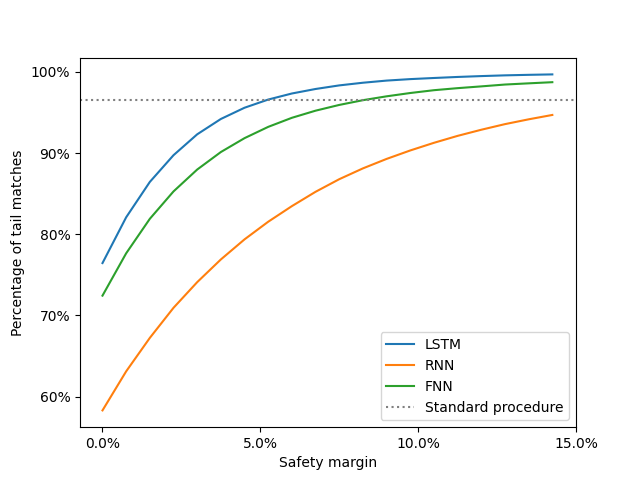
\includegraphics[width=0.48\textwidth]{../project2/figures/tailMatches/nnLN.png}
        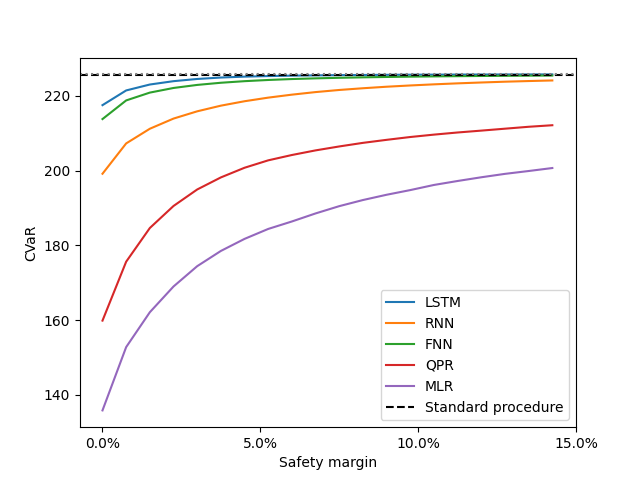
\includegraphics[width=0.48\textwidth]{../project2/figures/CVaR/allLN.png}
        \caption{Tail Matches and CVaR Predictions for DNN Metamodels}
    \end{figure}

    \begin{itemize}
        \item Traditional regression metamodels are \textbf{unable} to accurately identify tail scenarios even with high safety margins.
        \item LSTM metamodels surpasses the standard procedure with $5\%$ safety margin.
    \end{itemize}

    \note{We now consider the tail scenario identification and the CVaR estimation for the two-stage procedure. \\}
    \note{On the left is the tail scenario identification plot, and on the right is the plot of CVaR. \\}
    \note{We compare the two-stage procedure with the standard procedure. \\}
    \note{When colored lines cross the grey dashed line, it means that the metamodel is able to identify the tail scenarios as well as the standard procedure. \\}
    \note{And it should be able to estimate the CVaR as accurately as the standard procedure. \\}
    \note{We find that the LSTM metamodel is able to surpass the standard procedure on tail identification with a less than $5\%$ safety margin. \\}
    \note{However, the traditional regression metamodel is unable to identify the tail scenarios even with a high safety margin. \\}
    \note{A well-trained RNN is better than a FNN, but the poorly-trained RNN is far worse.}
    \note{The CVaR estimation plot shows similar results.}
        
\end{frame}

% \begin{frame}{Estimating CVaR}
    
%     \begin{figure}[H]
%         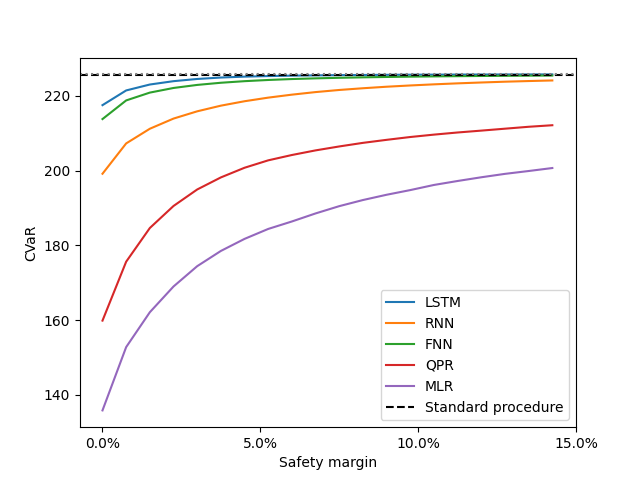
\includegraphics[width=0.48\textwidth]{../project2/figures/CVaR/allLN.png}
%         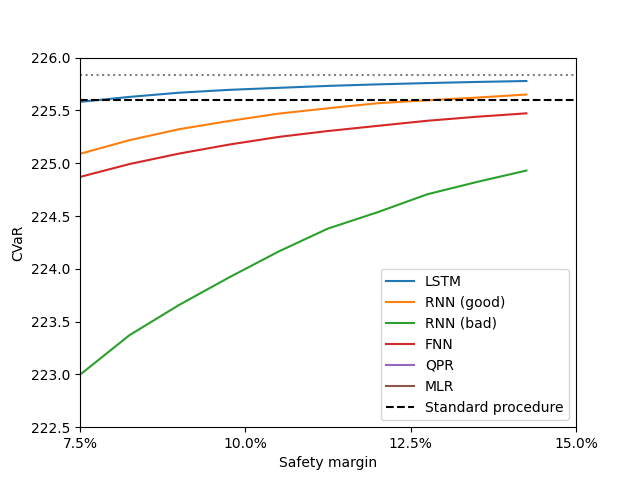
\includegraphics[width=0.48\textwidth]{../project2/figures/CVaR/zoomedLN.png}
%         \caption{CVaR estimation for DNN metamodels}
%     \end{figure}

%     \begin{itemize}
%         \item Traditional regression metamodels are \textbf{unable} to accurately estimate CVaR even with high safety margins.
%         \item LSTM surpasses the standard procedure with a \textbf{5\% safety margin}.
%         \item With a 95\% safety margin, any two-stage procedure produce the same CVaR estimate as a standard procedure.
%     \end{itemize}

%     \note{We now consider the CVaR estimation for the two-stage procedure. \\}
%     \note{On the left is the CVaR estimation for the all metamodels, and on the right is the zoomed-in version. \\}
%     \note{Their performance estimating CVaR is similar to their performance on tail identification. \\}
%     \note{The LSTM metamodel is able to surpass the standard procedure on CVaR estimation with a less than $5\%$ safety margin. \\}
%     \note{However, the traditional regression metamodel is unable to estimate the CVaR even with a high safety margin. \\}
%     \note{For the zoomed-in version, we can see that the LSTM metamodel is approaching CVaR of the standard procedure but not the true CVaR. \\}
%     \note{This is because in the second stage, the inner simulations are still not noiseless. \\}
%     \note{We use the same inner simulation for both the standard procedure and the two-stage procedure, which has 1000 inner replications for each outer scenario. \\}

% \end{frame}

\begin{frame}{Sensitivity Testing for DNNs}

    Simulation controls \textbf{noise level in training labels} and \textbf{number of training samples}.

    \vspace{10pt}
    
    $N'$ varies the noise level.

    \begin{itemize}
        \item   \textbf{Low noise labels}: $N' = 100$
        \item   \textbf{Medium noise labels}: $N' = 10$
        \item   \textbf{High noise labels}: $N' = 1$
    \end{itemize}

    \vspace{10pt}

    $M$ varies the number of training samples.

    \begin{itemize}
        \item $M \in \{10^2, 10^3, 10^4, 10^5\}$
    \end{itemize}

    \vspace{10pt}

    2 LSTMs of \textbf{different capacities} are examined based on their MSEs.

    \note{We now dig deeper into the research questions asked: how well do deep learning metamodels learn from noisy data? \\}
    \note{We study this phenomenon by considering the sensitivity testing for the DNN metamodels. \\}
    \note{The sensitivity of the DNN metamodels to the noise level in training labels and the number of training samples. \\}
    \note{In a simulation experiment, we can vary them to see how the DNN metamodels perform. \\}
    \note{We control the noise level in training labels by varying the number of inner replications $N'$. \\}
    \note{We control the number of training samples by varying the number of outer scenarios $M$. \\}
    \note{We consider two LSTM metamodels of different capacities because we want to see if the capacity of the metamodel matters for overfitting. \\}
    \note{The high-capacity LSTM metamodel has 10 times more parameters than the regular LSTM metamodel}

\end{frame}

% \begin{frame}{Noise Tolerance of DNNs}
    
%     \begin{table}[ht!]
%         \centering
%         \begin{tabular}{lccccc}
%             \toprule
%             \textbf{Model}      & \textbf{$N'$}         & \textbf{Training error}                & \textbf{Test error}               & \textbf{True error}\\
%             \midrule
%             LSTM                & $100$                & $0.075$         & $0.079$     & $0.063$ \\ 
%             High-capacity LSTM  & $100$                & $0.068$         & $0.102$     & $0.060$ \\
%             Average Difference  & $100$                & $-0.007$       & $0.023$     & $-0.003$ \\
%             \hline
%             LSTM                & $10$                 & $0.195$         & $0.193$     & $0.070$ \\
%             High-capacity LSTM  & $10$                 & $0.157$         & $0.199$     & $0.065$ \\
%             Average Difference  & $10$                 & $-0.038$       & $0.006$     & $-0.005$ \\
%             \hline
%             LSTM                & $1$                  & $1.366$         & $0.781$     & $0.129$ \\
%             High-capacity LSTM  & $1$                  & $1.354$         & $0.795$     & $0.149$ \\
%             Average Difference  & $1$                  & $-0.012$       & $0.014$     &\textcolor{color10_5}{$0.020$} \\
%             \bottomrule
%         \end{tabular}
%         \caption{MSEs of LSTM metamodels.}
%     \end{table}

%     \begin{itemize}
%         \item   Both LSTMs cut through the noise in training labels.
%         \item   Both LSTMs deteriorate dramatically on \textbf{high-noise} labels.
%         \item   High-capacity LSTM can tolerate \textbf{low} and \textbf{medium} label noise.
%     \end{itemize}

%     \note{This table shows the MSEs of the two LSTM metamodels on different datasets. \\}
%     \note{We also record the average difference in MSEs between the two LSTM metamodels. \\}
%     \note{Their difference indicates which LSTM is better at different noise levels. \\}
%     \note{The high-capacity LSTM is better at low and medium noise levels, while the regular LSTM is better at high noise levels. \\}
%     \note{This is because the high-capacity LSTM has more parameters and is therefore more flexible to fit the training data. \\}
%     \note{However, the regular LSTM is more robust to high noise levels. \\}
%     \note{We note that the high-capacity LSTM can tolerate quite a lot of noise in the training labels. \\}
%     \note{With only 10 inner replications, the high-capacity LSTM can still achieve a true MSE.}
%     \note{It is only when the labels become extremely noisy that the high-capacity LSTM deteriorates. $N=1$ is the most noise we are able to achieve in a simulation experiment.}

% \end{frame}

\begin{frame}{Noise Tolerance of DNNs}

    \begin{figure}[ht!]
        \centering
        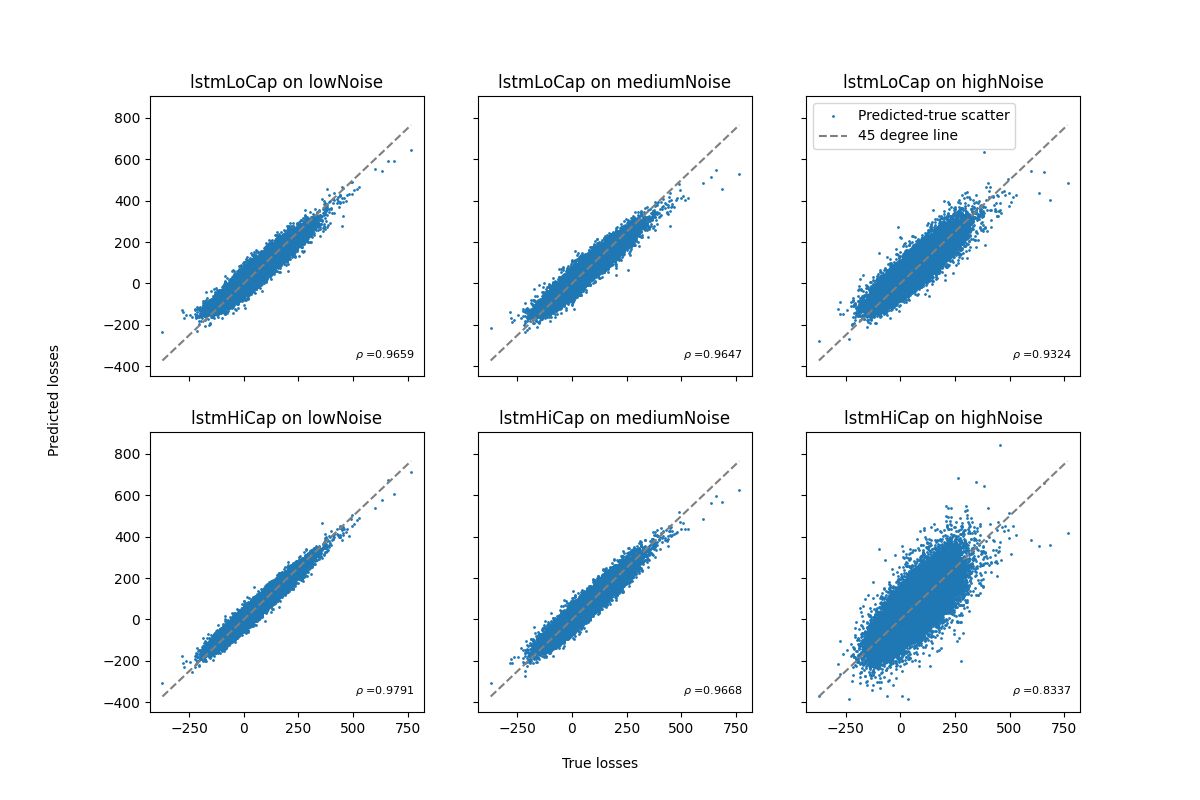
\includegraphics[width=\textwidth]{../project2/figures/qqPlots/lstmAll.png}
    \end{figure}

    \note{This figure shows the QQ plots of the two LSTM metamodels. \\}
    \note{We plot the predicted losses versus the true losses for both LSTMs and different noise levels. \\}
    \note{The high-capacity LSTM is better at low and medium noise levels, while the regular LSTM is better at high noise levels. \\}
    \note{We can see on the bottom right that the high-capacity LSTM has very poor performance.}

\end{frame}

% \begin{frame}{Sensitivity of Regular LSTM}

%     \begin{table}[ht!]
%         \centering
%         \begin{tabular}{lccccc}
%             \toprule
%                            & $N'=1$   & $N'=10$  & $N'=100$ & $N'=1000$\\
%             \midrule
%             $M = 100$      & \textcolor{color10_2}{$1.139$} & \textcolor{color10_3}{$0.229$} & \textcolor{color10_4}{$0.167$} & \textcolor{color10_5}{$0.158$} \\
%             $M = 1000$     & \textcolor{color10_3}{$0.559$} & \textcolor{color10_4}{$0.173$} & \textcolor{color10_5}{$0.123$} & \textcolor{color10_6}{$0.127$} \\
%             $M = 10000$    & \textcolor{color10_4}{$0.283$} & \textcolor{color10_5}{$0.115$} & \textcolor{color10_6}{$0.099$} & \textcolor{color10_7}{$0.097$} \\
%             $M = 100000$   & \textcolor{color10_5}{$0.129$} & \textcolor{color10_6}{$0.070$} & \textcolor{color10_7}{$0.063$} & \textcolor{color10_8}{$0.063$} \\
%             \bottomrule
%         \end{tabular}
%         \caption{MSE between regular LSTM's predicted losses and true losses.}
%     \end{table}

%     \begin{itemize}
%         \item   Same color $\rightarrow$ same total simulation budget.
%         \item   $N' = 10$ is a reasonable budget allocation for LSTM metamodels.
%     \end{itemize}

%     \note{This table shows the MSEs of the two LSTM metamodels on different datasets. \\}
%     \note{We modify $M$, the number of outer scenarios, and $N'$, the number of inner replications. \\}
%     \note{$M$ is the number of data points in the training set, and $N'$ is the noise level in the training labels. \\}
%     \note{We see similar patterns as in the previous table. \\}
%     \note{Additional findings being that the number of data points, $M$ also matters. \\}
%     \note{And it matters more for than $N'$ does. \\}
%     \note{In this table, the entries in the same diagonal represent the same total simulation budget. \\}
%     \note{It gives us a good indication of how much noise the LSTM metamodel can tolerate. \\}
%     \note{For a practical application, we almost want to increase $M$ as much as possible. \\}
%     \note{However, we can see that in the diagonal of red color, we should keep $N'$ at 10 and not lower it to 1. \\}
%     \note{We don't want the training labels to be too noisy. \\}
%     \note{If we increase $M$ too much, the performance of the regular LSTM will also deteriorate. \\}

% \end{frame}

\begin{frame}{Sensitivity of High-capacity LSTM}

    \begin{table}[ht!]
        \centering
        \begin{tabular}{lccccc}
            \toprule
            & $N'=1$ & $N'=10$  & $N'=100$ & $N'=1000$\\
            \midrule
            $M = 100$      & \textcolor{color10_2}{$0.764$} & \textcolor{color10_3}{$0.408$} & \textcolor{color10_4}{$0.131$} & \textcolor{color10_5}{$0.087$} \\
            $M = 1000$     & \textcolor{color10_3}{$0.878$} & \textcolor{color10_4}{$0.367$} & \textcolor{color10_5}{$0.156$} & \textcolor{color10_6}{$0.087$} \\
            $M = 10000$    & \textcolor{color10_4}{$0.351$} & \textcolor{color10_5}{$0.147$} & \textcolor{color10_6}{$0.064$} & \textcolor{color10_7}{$0.063$} \\
            $M = 100000$   & \textcolor{color10_5}{$0.149$} & \textcolor{color10_6}{$0.065$} & \textcolor{color10_7}{$0.060$} & \textcolor{color10_8}{$0.038$} \\
            \bottomrule
        \end{tabular}
        \caption{MSE between high-capacity LSTM's predicted losses and true losses.}
    \end{table}

    \begin{itemize}
        \item   Same color $\rightarrow$ same total simulation budget.
        \item   $N' = 10$ is a reasonable budget allocation for LSTM metamodels.
    \end{itemize}

    \note{This table shows the MSEs of the two LSTM metamodels on different datasets. \\}
    \note{We modify $M$, the number of outer scenarios, and $N'$, the number of inner replications. \\}
    \note{$M$ is the number of data points in the training set, and $N'$ is the noise level in the training labels. \\}
    \note{We have additional findings that the number of data points, $M$ also matters. \\}
    \note{And it matters more for than $N'$ does. \\}
    \note{In this table, the entries in the same diagonal represent the same total simulation budget. \\}
    \note{It gives us a good indication of how much noise the LSTM metamodel can tolerate. \\}
    \note{For a practical application, we almost want to increase $M$ as much as possible. \\}
    \note{However, we can see that in the diagonal of red color, we should keep $N'$ at 10 and not lower it to 1. \\}
    \note{We don't want the training labels to be too noisy.}
    
\end{frame}

\begin{frame}{Single-Stage Procedure}

    \begin{figure}[ht!]
        \centering
        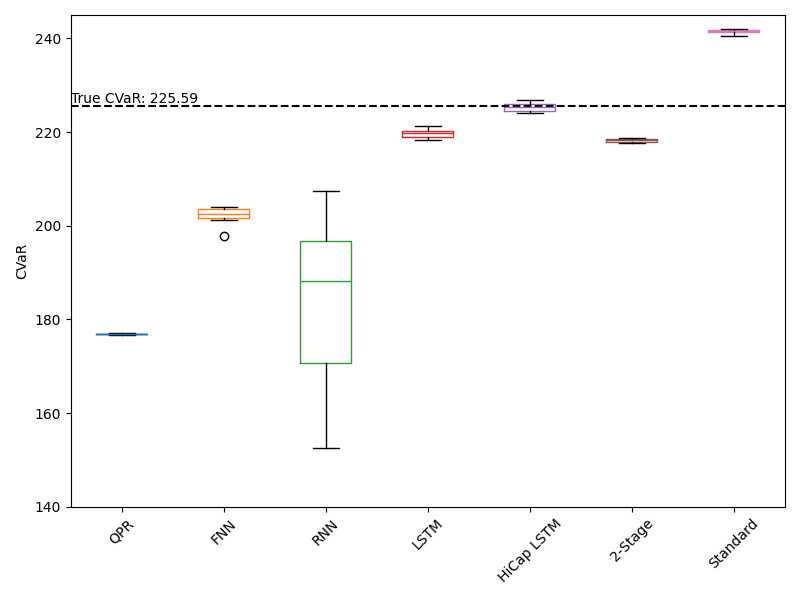
\includegraphics[width=0.6\textwidth]{../project2/figures/singleStage/CVaRmediumNoise.png}
        % 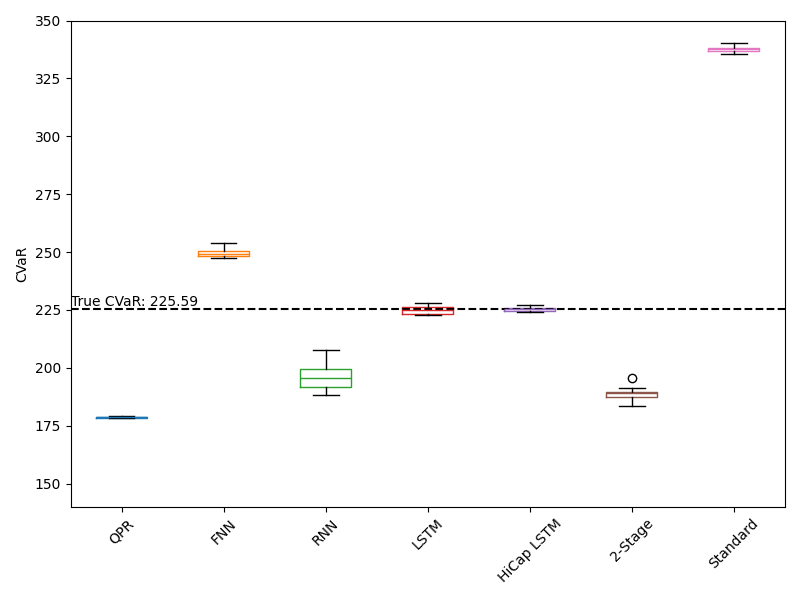
\includegraphics[width=0.48\textwidth]{../project2/figures/singleStage/CVaRhighNoise.png}
        \caption{CVaR estimates of single-stage procedures with $N' = 10$.}
    \end{figure}

    \begin{itemize}
        \item   The single-stage procedure outperforms the two-stage procedure.
        \item   $N' = 10$ is a reasonable budget allocation.
    \end{itemize}

    \note{This figure shows the CVaR estimates of the single-stage procedure. \\}
    \note{We compare it with the two-stage procedure using regular LSTM metamodel with no safety margin. So we are using the 5\% metamodel predicted tails to estimate the 95\% CVaR with extensive simulation in stage 2. \\}
    \note{The single-stage procedure with LSTM metamodels outperforms the two-stage procedure when noise level is moderate. \\}
    \note{Due to its design, the single-stage procedure is more efficient than the two-stage procedure. \\}
    \note{Setting $N' = 10$ is a reasonable budget allocation for the single-stage procedure. \\}
    \note{Further decreasing $N'$ to 1 deteriorates the performance of the single-stage procedure. But it is worth noting that the 2-stage procedure can overcome this issue by increasing the safety margin. \\}

\end{frame}

% \begin{frame}{Convergence Analysis}

%     For each $\Gamma$, the best performing metamodel is used.

%     \begin{itemize}
%         \item   Maximum number of outer scenarios $M = 10^5$.
%     \end{itemize}

%     \begin{figure}[ht!]
%         \centering
%         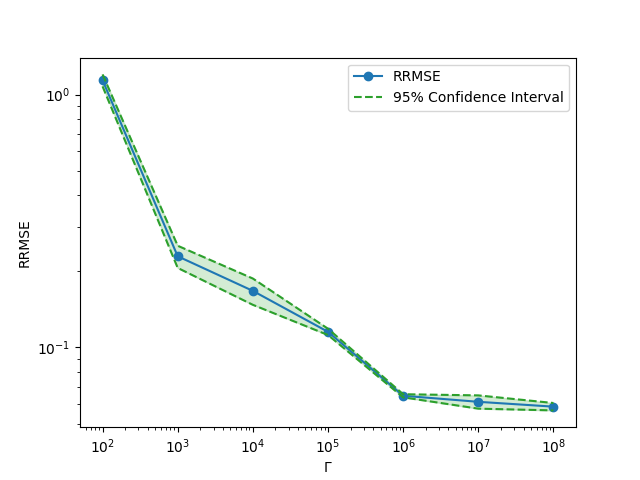
\includegraphics[width=0.48\textwidth]{../project2/figures/singleStage/MSEConvergence_lstmLoCap.png}
%         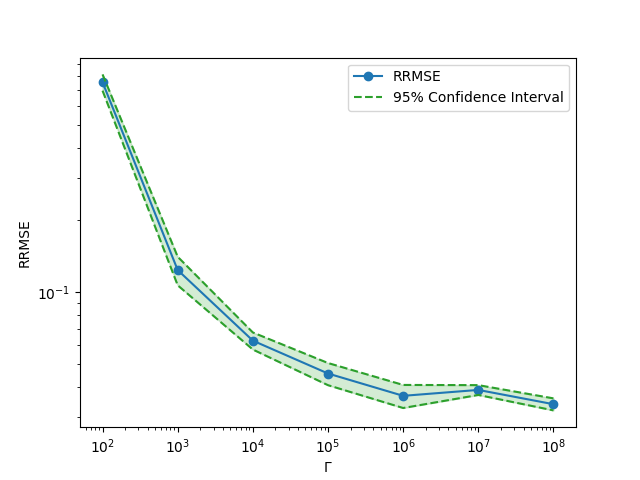
\includegraphics[width=0.48\textwidth]{../project2/figures/singleStage/MSEConvergence_lstmHiCap.png}
%         \caption{Empirical convergence of CVaR for single-stage procedures with LSTM metamodels (left: regular LSTM. right: high-capacity LSTM).}
%     \end{figure}

%     \begin{itemize}
%         \item   Minimal effect of increasing $N'$ on CVaR estimation.
%         \item   Similar behavior as regression metamodels ($d=20$) in the previous section.
%     \end{itemize}
    
%     \note{This figure shows the empirical convergence of CVaR for the single-stage procedure with LSTM metamodels. \\}
%     \note{We use the best performing metamodel for each $\Gamma$. \\}
%     \note{The maxmium number of outer scenarios we can afford is $M = 10^5$. \\}
%     \note{For budget larger than $10^6$, we uses higher $N'$ and keeping the maximum number of outer scenarios $M$ fixed at $10^5$. \\}
%     \note{The regular LSTM plot on the left between $10^3$ and $10^6$ offers a good indication of how empirically LSTM-based CVaR estimation converges to the true CVaR. \\}
%     \note{We can further investigate the convergence rate by plotting the RRMSE for $M$ and $N$ separately. \\}
    

% \end{frame}

\begin{frame}{Convergence Analysis}
    \begin{figure}[ht!]
        \centering
        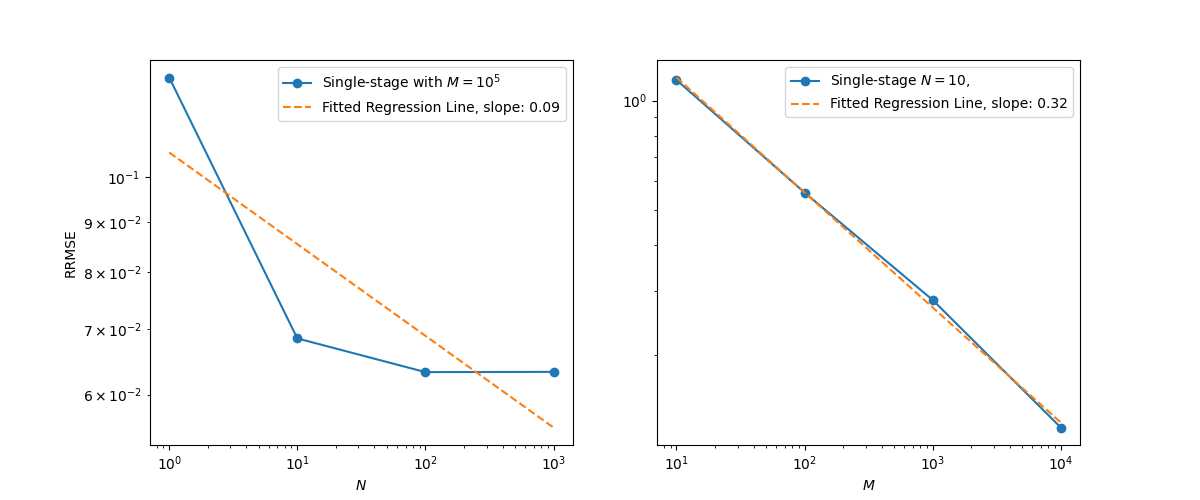
\includegraphics[width=\textwidth]{../project2/figures/singleStage/MSEConvergence_lstmLoCap_MN.png}
        \caption{Empirical convergence of the single-stage procedure with a LSTM metamodel.} 
    \end{figure}

    \begin{itemize}
        \item   Minimal effect of increasing $N'$ on CVaR estimation.
        \item   For a given $\Gamma$, set $N'$ constant and allocate budget to outer simulations.
    \end{itemize}

    \note{This figure shows the empirical convergence of the single-stage procedure with LSTM metamodels when only $M$ or $N'$ is varied. \\}
    \note{On the left, we fix $M=10^5$ and vary $N'$. \\}
    \note{There is no significant difference to further increase $N'$ when $N' \geq 10$. \\}
    \note{On the right, we fix $N'=10$ and vary $M$. \\}
    \note{We can see that the convergence rate is around $O(M^{-2/3})$. \\}
    \note{This finding is consistent with our previous analysis on the sensitivity of LSTM metamodels to data quality and data quantity. \\}
    \note{Once the quality is good enough, the quantity is more important. \\}

\end{frame}

\begin{frame}{Conclusion}

    \textbf{Key Findings:}
    \begin{itemize}
        \item   LSTMs are \textbf{resilient} to moderate levels of noise in training labels.
        \item   DNNs can learn \textbf{true} complex dynamic hedging model.
        \item   Two-stage procedure addresses regulatory concerns.
        \item   Single-stage procedure is \textbf{efficient}.
    \end{itemize}

    \vspace{10pt}

    \textbf{Future Directions:}
    \begin{itemize}
        \item   Apply DNNs to other risk management tasks.
        \item   Fast adaptation to new contracts/market conditions.
    \end{itemize}

    \note{In this project, we present our extensive research into LSTM metamodels in a simulation setting.\\}
    \note{Our findings demonstrate that LSTMs can effectively learn complex hedging strategies even with noisy training data.\\}
    \note{The single-stage procedure offers an excellent balance of efficiency and accuracy for practical applications.\\}
    \note{We've shown that allocating computational budget to increase outer scenarios rather than inner simulations yields better results.\\}
    \note{These insights provide valuable guidance for implementing machine learning in financial risk management.\\}
    \note{For the research directions, we can apply deep neural network metamodels to other actuarial applications.\\}
    \note{We can also apply transfer learning to speed up the training process for deep neural network metamodels.\\}
    
\end{frame}


\section[TL for DNN Metamodels]{Transfer Learning for Rapid Adaptation of DNN Metamodels}

\begin{frame}{Transfer Learning for Rapid Adaptation of DNN Metamodels}

    \textbf{Problem:} Updating models for new conditions is expensive.
    \begin{itemize}
        \item   Full retraining takes too much time.
        \item   New VA contracts need quick model updates.
        \item   Need balance between speed and accuracy.
    \end{itemize}

    \vspace{10pt}

    \textbf{Solution:} Transfer learning for faster model adaptation.

    \begin{itemize}
        \item   Train first on existing contract data.
        \item   Update with small amount of new contract data.
        \item   Reuse knowledge between similar contracts.
        \item   Benefits:
            \begin{itemize}
                \item   Faster training.
                \item   Less data needed.
            \end{itemize}
    \end{itemize}

    \note{In this project, we propose a transfer learning framework for rapid adaptation of deep neural network metamodels in VA dynamic hedging.\\ }
    \note{The problem is the same as the previous project. We want to use deep neural network metamodels to approximate the complex simulation model that involves dynamic hedging.\\}
    \note{The difference is that we want to use transfer learning to speed up the training process.\\}
    \note{This can be beneficial for the practical applications.\\}
    \note{Firstly, new VA contracts are continuously issued.\\}
    \note{Secondly, market conditions are changing.\\}
    \note{Thirdly, the computational budget is limited.\\}
    \note{Transfer learning can help us to adapt to the new market conditions quickly and efficiently.\\}
    \note{We can pre-train the deep neural network metamodel on a large dataset of VA contracts with abundant simulation data.\\}
    \note{Then, we can fine-tune the metamodel on a smaller dataset of new VA contracts with limited data.\\}
    \note{The data is often limited for new VA contracts as simulation is expensive to run.\\}
    \note{The shared features between VA contracts can be leveraged to speed up the training process.\\}
    \note{We can also transfer the knowledge to other contract types.\\}
    \note{When a new VA contract is issued, we can use transfer learning to adapt the metamodel to the new contract quickly.\\}

\end{frame}


\begin{frame}{Transfer Learning Framework}

    \textbf{Key Components:}
    \begin{itemize}
        \item   \textbf{Domain} $\mathcal{D}$: feature space $\mathcal{X}$ + probability distribution $F$
        \item   \textbf{Task} $\mathcal{T}$: label space $\mathcal{Y}$ + predictive function $f: \mathcal{X} \rightarrow \mathcal{Y}$
    \end{itemize}

    \vspace{10pt}
    \textbf{Source vs. Target:}
    \begin{itemize}
        \item   \textbf{Source:} $\mathcal{D}_{\text{So}} = \{\mathcal{X}_{\text{So}}, F_{\text{So}}(X)\}$
        \item   \textbf{Target:} $\mathcal{D}_{\text{Ta}} = \{\mathcal{X}_{\text{Ta}}, F_{\text{Ta}}(X)\}$
    \end{itemize}

    \vspace{10pt}
    \textbf{Our Goal:}
    \begin{itemize}
        \item   \textbf{Input features} $X$: risk factors from outer simulation
        \item   \textbf{Output labels} $L$: contract losses
        \item   \textbf{Source and target}: from VAs with abundant simulation data to new VAs with limited data
        \item   \textbf{Goal}: improve $f_{\text{Ta}}(\cdot)$ using knowledge from $\mathcal{D}_{\text{So}}$ and $f_{\text{So}}(\cdot)$
    \end{itemize}

    \note{Transfer learning provides a formal framework for adapting models from one domain to another.\\}
    \note{The domain consists of a feature space and a probability distribution over that space.\\}
    \note{In our context, the feature space includes risk factors from the outer simulation.\\}
    \note{It is equipped with a probability distribution that describes the joint distribution of the risk factors.\\}
    \note{We don't know the exact joint distribution of the risk factors, but we can simulate outer scenarios from it using monte carlo simulation.\\}
    \note{The task consists of a label space and a predictive function mapping features to labels.\\}
    \note{For VA contracts, our labels are the contract losses under different scenarios.\\}
    \note{The source domain typically has abundant data - this could be existing VA contracts with extensive simulation data.\\}
    \note{The target domain has limited data - new VA contracts or existing contracts under new market conditions.\\}
    \note{Our goal is to leverage knowledge from the source domain to improve prediction in the target domain.\\}
    \note{This is particularly valuable when simulation data is expensive to generate for new contracts.\\}
    \note{The transfer learning approach allows us to maintain accuracy while significantly reducing computational requirements.}

\end{frame}

\begin{frame}{Transfer Learning Techniques}

    \textbf{Common Techniques:}
    \begin{itemize}
        \item   \textbf{Fine-tuning:} a model pre-trained on a source task is used as a starting point for a target task.
        \item   \textbf{Layer freezing:} only part of the model is fine-tuned.
    \end{itemize}

    \vspace{10pt}

    \textbf{Key considerations:} similarity between source and target tasks

    \vspace{10pt}

    \textbf{Experiment Design:}
    \begin{itemize}
        \item   Source domain (50000 samples): GMMB with no lapse and GMMB with static lapse
        \item   Target domain (2000 samples): GMMB with dynamic lapse
    \end{itemize}


    \note{Fine-tuning involves using a pre-trained model as a starting point for a new task.\\}
    \note{For VA contracts, we can fine-tune models between different contract types or market conditions.\\}
    \note{Layer freezing is a technique where we keep some layers of the pre-trained model fixed.\\}
    \note{Typically, early layers capture general features while later layers are more task-specific.\\}
    \note{By freezing early layers, we preserve general knowledge while adapting task-specific layers.\\}
    \note{In our experiment, we use the same model architecture for all tasks. \\}
    \note{Metamodels are trained with 50,000 samples on the source domain before transferring to the target domain with only 2000 samples. \\}
    \note{We progress from simpler to more complex models (No lapse → Static → Dynamic). \\}
    \note{The experiments are designed to evaluate how similarity between source and target affects transfer efficiency. \\}
    \note{This is another attempt to use simulation models as data generating processes to examine deep neural networks. \\}
    \note{By examining the transfer learning performance, we can gain insights into which parts of the neural network are transferable, or more generally, which layers of the neural network learn which features of the VA contracts. }

\end{frame}

% \begin{frame}{Fine-tuning Algorithm for LSTM Metamodels in VA Hedging}

%     \begin{algorithm}[H]
%         \caption{Fine-tuning Algorithm for LSTM Metamodels in VA Hedging}
%         \begin{algorithmic}[1]
%             \STATE \textbf{Input:} $\mathcal{D}_{\text{So}} = \{(X_{\text{So}}^{(i)}, L_{\text{So}}^{(i)})\}_{i=1}^{M_{\text{So}}}$ , $\mathcal{D}_{\text{Ta}} = \{(X_{\text{Ta}}^{(i)}, L_{\text{Ta}}^{(i)})\}_{i=1}^{M_{\text{Ta}}}$, $\alpha_{\text{So}}$, and $\alpha_{\text{Ta}}$.
%             \STATE Train a LSTM metamodel $f_{\text{So}}(\cdot; \theta_{\text{So}})$ on $\mathcal{D}_{\text{So}}$:
%             \begin{equation*}
%                 \theta_{\text{So}} = \min_{\theta} \frac{1}{M_{\text{So}}} \sum_{i=1}^{M_{\text{So}}} \left( f_{\text{So}}(X_{\text{So}}^{(i)}; \theta) - L_{\text{So}}^{(i)} \right)^2
%             \end{equation*}
%             \STATE Initialize the target metamodel parameters $\theta_{\text{Ta}}$ using the pre-trained metamodel parameters:
%             \begin{equation*}
%                 \theta_{\text{Ta}} \gets \theta_{\text{So}}
%             \end{equation*}
%             \STATE Fine-tune the entire LSTM metamodel $f_{\text{Ta}}(\cdot; \theta_{\text{Ta}})$ on the target dataset $\mathcal{D}_{\text{Ta}}$ using a smaller learning rate $\alpha_{\text{Ta}}$:
%             \begin{equation*}
%                 \theta_{\text{Ta}} = \min_{\theta} \frac{1}{M_{\text{Ta}}} \sum_{i=1}^{M_{\text{Ta}}} \left( f_{\text{Ta}}(X_{\text{Ta}}^{(i)}; \theta) - L_{\text{Ta}}^{(i)} \right)^2
%             \end{equation*}
%             \STATE \textbf{Output:} Final adapted LSTM metamodel $f_{\text{Ta}}(\cdot; \theta_{\text{Ta}})$ for the target task
%         \end{algorithmic}
%     \end{algorithm}
    
%     \note{This algorithm outlines the fine-tuning process for LSTM metamodels in VA hedging. \\}
%     \note{We start with a source dataset $\mathcal{D}_{\text{So}}$ and a target dataset $\mathcal{D}_{\text{Ta}}$. \\}
%     \note{First, we train the source model on the larger source dataset. \\}
%     \note{Then we initialize the target model with the pre-trained weights from the source model. \\}
%     \note{The key is using a smaller learning rate $\alpha_{\text{Ta}}$ during fine-tuning. \\}
%     \note{This prevents catastrophic forgetting of useful features learned from the source task. \\}
%     \note{The entire model is updated during fine-tuning, unlike layer freezing. \\}
%     \note{This approach works well when source and target tasks are similar. \\}
%     \note{For VA contracts, this might mean transferring between similar contract types. \\}
%     \note{The effectiveness depends on the similarity between source and target domains. \\}
% \end{frame}

% \begin{frame}{Layer Freezing Algorithm for LSTM Metamodels in VA Hedging}

%     \begin{algorithm}[H]
%         \caption{Layer Freezing Algorithm for LSTM Metamodels in VA Hedging}
%         \begin{algorithmic}[1]
%             \STATE \textbf{Input:} $\mathcal{D}_{\text{So}} = \{(X_{\text{So}}^{(i)}, L_{\text{So}}^{(i)})\}_{i=1}^{M_{\text{So}}}$ , $\mathcal{D}_{\text{Ta}} = \{(X_{\text{Ta}}^{(i)}, L_{\text{Ta}}^{(i)})\}_{i=1}^{M_{\text{Ta}}}$, $\alpha_{\text{So}}$, and $\alpha_{\text{Ta}}$.
%             \STATE Train LSTM model $f_{\text{So}}(\cdot; \theta_{\text{So}})$ on $\mathcal{D}_{\text{So}}$.
%             \STATE Initialize the target model parameters $\theta_{\text{Ta}} = [\theta_0, \theta_1]$ using the pre-trained source model parameters $\theta_{\text{So}}$:
%             \begin{equation*}
%                 \theta_{\text{Ta}} \gets \theta_{\text{So}} = [\theta_0, \theta_1]
%             \end{equation*}
%             \STATE Freeze the parameters of the shared layers $\theta_0$ and fine-tune the trainable layers $\theta_1$ on the target dataset $\mathcal{D}_{\text{Ta}}$:
%             \begin{equation*}
%                 \theta_{\text{Ta}} = \min_{\theta_1} \frac{1}{M_{\text{Ta}}} \sum_{i=1}^{M_{\text{Ta}}} \left( f_{\text{Ta}}(X_{\text{Ta}}^{(i)}; [\theta_0, \theta_1]) - L_{\text{Ta}}^{(i)} \right)^2
%             \end{equation*}
%             \STATE \textbf{Output:} Adapted model $f_{\text{Ta}}(\cdot; \theta_{\text{Ta}})$ for the target task.
%         \end{algorithmic}
%     \end{algorithm}

%     \note{The difference between the fine-tuning and layer freezing algorithms is that the parameters of the shared layers are frozen in the layer freezing algorithm. \\}
%     \note{This allows us to preserve the general knowledge learned from the source task while adapting the task-specific layers. \\}
%     \note{Layer freezing is particularly effective when the source and target tasks share similar low-level features. \\}
%     \note{In the context of VA contracts, this might mean transferring between contracts with similar underlying asset dynamics. \\}
%     \note{The choice of which layers to freeze is critical - typically early layers capture general features. \\}
%     \note{Later layers tend to be more task-specific and should be fine-tuned. \\}
%     \note{This approach preserves the feature extraction capabilities learned from the source task. \\}
%     \note{It's computationally efficient as fewer parameters need to be updated during training. \\}
%     \note{Layer freezing can help prevent overfitting when the target dataset is small. \\}
%     \note{The tradeoff is less flexibility compared to full fine-tuning. \\}
%     \note{For VA contracts with significantly different features, fine-tuning may be more appropriate. \\}
%     \note{Empirical testing is often needed to determine the optimal freezing strategy. \\}

% \end{frame}

% \begin{frame}{Multi-task Learning Algorithm for LSTM Metamodels in VA Hedging}

%     \begin{algorithm}[H]
%         \caption{Multi-task Learning Algorithm for LSTM Metamodels in VA Hedging}
%         \begin{algorithmic}[1] \label{alg3:multiTaskLearning}
%             \STATE \textbf{Input:} learning rate $\alpha$, set of $K$ tasks $\{\mathcal{T}_k\}_{k=1}^K$ with datasets $\mathcal{D}_k = \{(X_k^{(i)}, L_k^{(i)})\}_{i=1}^{M_k}$, task-specific parameters $\theta_k$ for each task $k$, and shared parameters $\theta_0$.
        
%             \STATE Train the multi-head LSTM metamodel on all $K$ tasks simultaneously by minimizing the multi-task loss function:
%             \begin{equation} \label{eq3:multiTaskLoss}
%                 \min_{\theta_0, \{\theta_k\}_{k=1}^K} \sum_{k=1}^K \frac{1}{M_k} \sum_{i=1}^{M_k} \left( f_i(X_k^{(i)}; \theta_0, \theta_k) - L_k^{(i)} \right)^2
%             \end{equation}
        
%             \STATE Update both the shared parameters $\theta_0$ and task-specific parameters $\{\theta_k\}_{k=1}^K$ simultaneously using backpropagation and gradient descent with learning rate $\alpha$.
            
%             \STATE \textbf{Output:} Trained multi-task metamodel $f(\cdot; \theta_0, \{\theta_k\}_{k=1}^K)$ for all $K$ tasks
%         \end{algorithmic}
%     \end{algorithm}

%     \note{Multi-task learning allows simultaneous training on multiple VA contract types. \\}
%     \note{The algorithm shares parameters across tasks while maintaining task-specific components. \\}
%     \note{This approach leverages the common underlying financial and mathematical structures. \\}
%     \note{The shared parameters $\theta_0$ capture general features applicable to all contracts. \\}
%     \note{Task-specific parameters $\theta_k$ adapt to the unique characteristics of each contract. \\}
%     \note{The loss function balances performance across all tasks. \\}
%     \note{This is particularly valuable when data for some contract types is limited. \\}
%     \note{Multi-task learning can improve generalization compared to single-task models. \\}
%     \note{It reduces the risk of overfitting on smaller datasets. \\}
%     \note{For VA contracts, this enables efficient modeling of GMMB and GMWB simultaneously. \\}
%     \note{The approach is scalable to more than two contract types. \\}
%     \note{Implementation requires careful balancing of task contributions to prevent domination. \\}
%     \note{Computational efficiency is achieved through shared feature extraction. \\}

% \end{frame}

% \begin{frame}{Multi-task Learning}
%     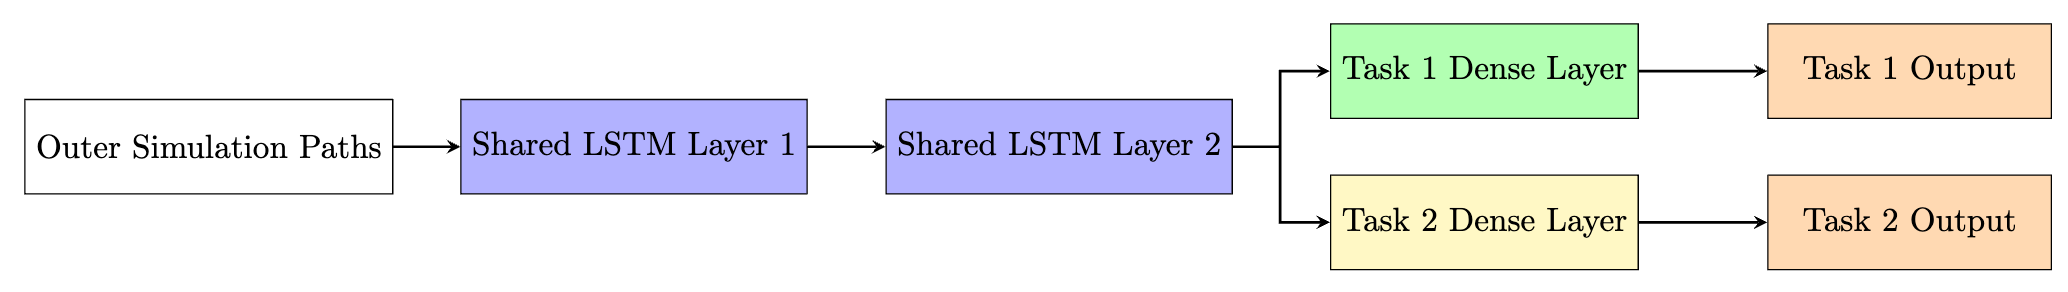
\includegraphics[width=0.9\textwidth]{../project3/figures/mtl.png}
    
%     \begin{itemize}
%         \item LSTM layers shared across multiple tasks
%         \item Task-specific fully connected layers
%         \item Objective: Minimize sum of loss functions across all tasks
%     \end{itemize}
    
%     \note{Multi-task learning offers an alternative approach to transfer learning. \\}
%     \note{Instead of sequential knowledge transfer, we train on multiple contract types simultaneously. \\}
%     \note{The shared LSTM layers capture common features across different VA contracts. \\}
%     \note{Task-specific layers then specialize for each contract type's unique characteristics. \\}
%     \note{We will examine whether this approach can be more efficient than training separate models for each contract type. \\}

% \end{frame}

% \begin{frame}{Experiment Setup}

%     \begin{table}[ht!] 
%         \centering
%         \begin{tabular}{lcccc} 
%         \toprule
%         \textbf{Contract} & \textbf{Asset Model} & \textbf{Lapse} & \textbf{$M_{\text{So}}$}  & \textbf{$M_{\text{Ta}}$}\\
%         \midrule
%         GMMB & GBM & No lapse & 50000 & N/A \\
%         GMMB & RS-GBM & No lapse & 50000 & 2000 \\
%         GMMB & RS-GBM & Static lapse & 50000 & 2000 \\
%         GMMB & RS-GBM & Dynamic lapse & 50000 & 2000 \\
%         GMWB & RS-GBM & Dynamic lapse & N/A & 2000 \\
%         \bottomrule
%         \end{tabular}
%         \caption{VA Contracts for Transfer Learning Experiments}
%     \end{table}

%     We aim to examine the performance of TL techniques
%     \begin{itemize}
%         \item   learning the lapse features,
%         \item   learning the dynamic lapse, and 
%         \item   transferring to other contract types.
%     \end{itemize}


%     \note{We use a variety of VA contracts with different features to test transfer learning. \\}
%     \note{The source model ($M_{\text{So}}$) is trained with 50,000 samples for comprehensive learning. \\}
%     \note{The target model ($M_{\text{Ta}}$) uses only 2,000 samples to simulate limited data scenarios. \\}
%     \note{We progress from simpler to more complex models (No lapse → Static → Dynamic). \\}
%     \note{We examine both within-contract transfer (GMMB to GMMB with different features) and cross-contract transfer (GMMB to GMWB). \\}
%     \note{All training data is generated using 100 inner replications for consistency. \\}
%     \note{We compare fine-tuning and layer freezing as two primary transfer learning approaches. \\}
%     \note{The experiments are designed to evaluate how similarity between source and target affects transfer efficiency. \\}
%     \note{This is another attempt to use simulation models as data generating processes to examine deep neural networks. \\}
%     \note{By examining the transfer learning performance, we can gain insights into which parts of the neural network are transferable, or more generally, which layers of the neural network learn which features of the VA contracts. \\}

% \end{frame}




% \begin{frame}{The Effect of Number of Training Samples}
%     \begin{figure}[ht]
%         \centering
%         \begin{subfigure}{0.48\textwidth}
%             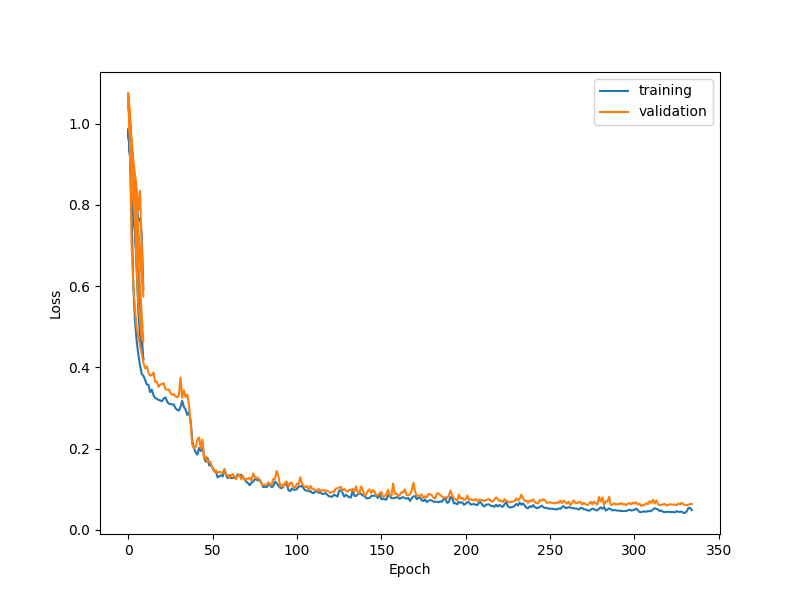
\includegraphics[width=\textwidth]{../project3/figures/figure1a.png}
%             \caption{50000 samples}
%         \end{subfigure}
%         \begin{subfigure}{0.48\textwidth}
%             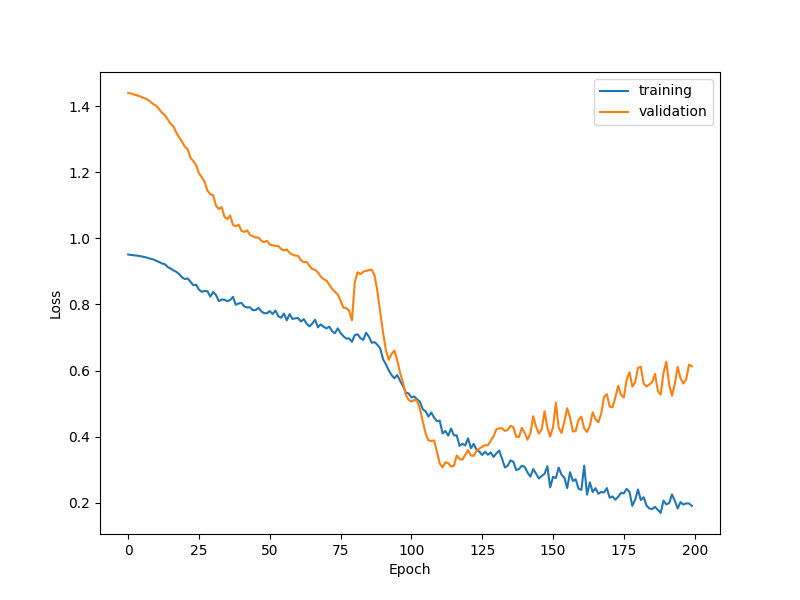
\includegraphics[width=\textwidth]{../project3/figures/figure1b.png}
%             \caption{2000 samples}
%         \end{subfigure}
%         \caption{Learning curves of GMMB contracts with static lapse}
%     \end{figure}

%     \note{We first examine the effect of the number of training samples on the convergence of the model. \\}
%     \note{There is no transfer learning in this experiment. \\}
%     \note{With 50,000 training samples, the model converges quickly to a low MSE. \\}
%     \note{With only 2,000 samples, convergence is slower and less stable. \\}
%     \note{Limited data scenarios are common in practice due to computational constraints. \\}
%     \note{The difference in performance highlights the need for transfer learning techniques. \\}
%     \note{More training data leads to better generalization and lower prediction error. \\}
%     \note{The figure on the right shows the challenge of training complex models with limited data. \\}
%     \note{This motivates our exploration of transfer learning to improve performance with limited data. \\}


% \end{frame}
    


% \begin{frame}{Learning Lapse Features using Transfer Learning}

%     \begin{figure}[ht]
%         \centering
%         \begin{subfigure}{0.48\textwidth}
%             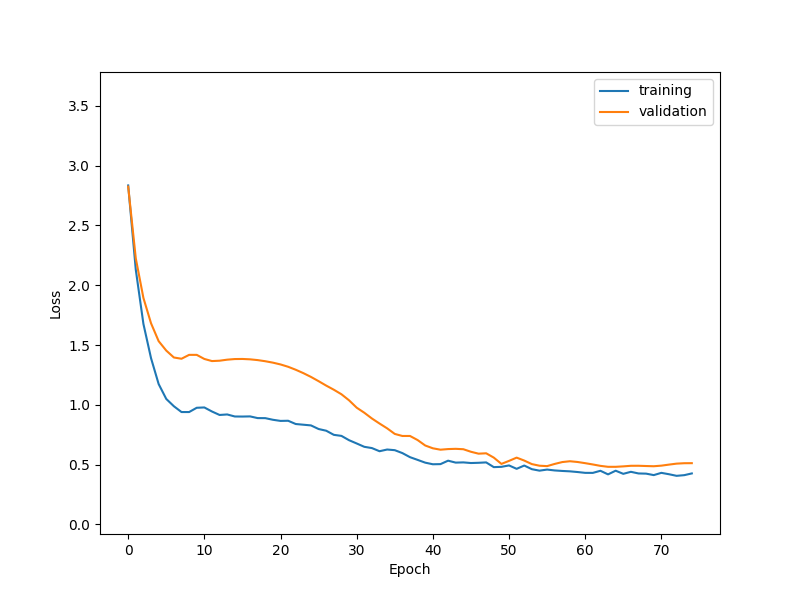
\includegraphics[width=\textwidth]{../project3/figures/figure1c.png}
%             \caption{Fine-tuning}
%         \end{subfigure}
%         \begin{subfigure}{0.48\textwidth}
%             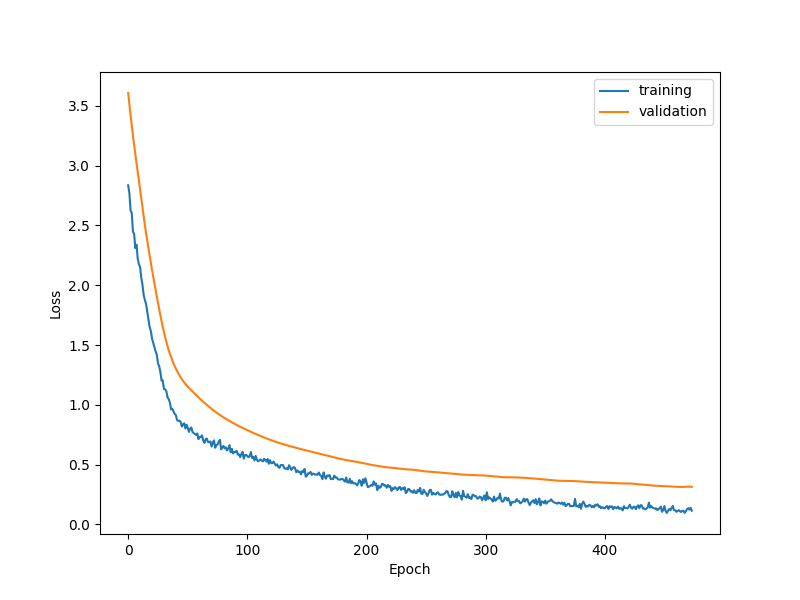
\includegraphics[width=\textwidth]{../project3/figures/figure1d.png}
%             \caption{Layer Freezing}
%         \end{subfigure}
%         \caption{Learning curves of GMMB contracts with static lapse}
%     \end{figure}

%     \note{This slide demonstrates the effectiveness of transfer learning techniques. \\}
%     \note{Fine-tuning (left) allows all model parameters to be updated during training on the target task. \\}
%     \note{Layer freezing (right) keeps early layers fixed and only updates later layers. \\}
%     \note{Both transfer learning approaches show significant improvement over training from scratch. \\}
%     \note{With only 2,000 samples, transfer learning achieves much lower MSE values. \\}
%     \note{Fine-tuning also converges fast but layer freezing shows more stability. \\}
%     \note{The knowledge transferred from the source model (no lapse) helps the model learn static lapse features. \\}
%     \note{Transfer learning reduces overfitting and improves generalization with limited data. \\}
%     \note{Here, we are only learning the lapse feature. \\}
%     \note{This demonstrates how knowledge from one VA contract can be leveraged for another when the difference between the source and target is small. \\}
    
% \end{frame}    
    
% \begin{frame}{Learning Curves: Learning Dynamic Lapse}

%     \begin{figure}[ht]
%         \centering
%         \begin{subfigure}{0.48\textwidth}
%             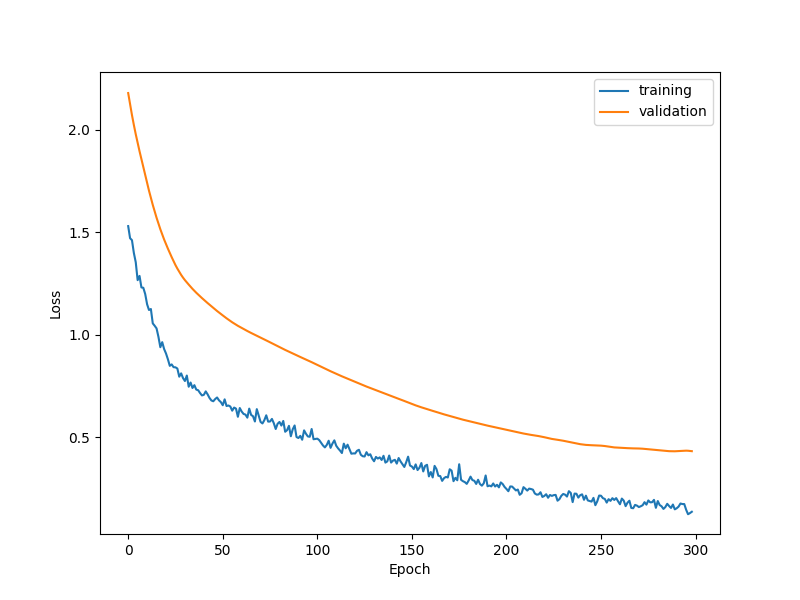
\includegraphics[width=\textwidth]{../project3/figures/figure2a.png}
%             \caption{No Lapse}
%         \end{subfigure}
%         \begin{subfigure}{0.48\textwidth}
%             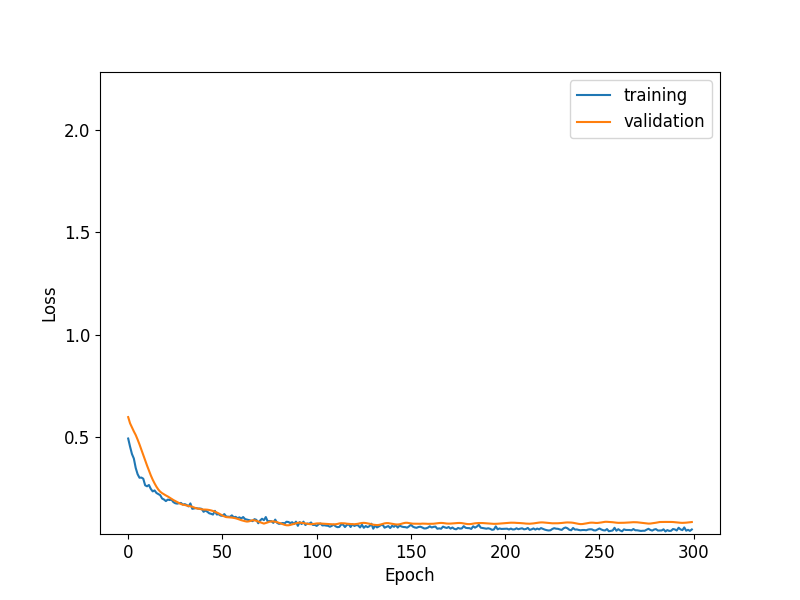
\includegraphics[width=\textwidth]{../project3/figures/figure2b.png}
%             \caption{Static Lapse}
%         \end{subfigure}
%         \caption{Learning curves of GMMB contracts with dynamic lapse}
%     \end{figure}

%     \note{This slide shows how transfer learning performs when learning dynamic lapse features. \\}
%     \note{The left figure shows transfer from a model trained on contracts with no lapse. \\}
%     \note{The right figure shows transfer from a model trained on contracts with static lapse. \\}
%     \note{We observe that the source model's similarity to the target task significantly impacts transfer learning effectiveness. \\}
%     \note{Transfer from static lapse (right) performs much better than transfer from no lapse (left). \\}
%     \note{This demonstrates the importance of task similarity in transfer learning. \\}
%     \note{When source and target domains are more similar (static to dynamic lapse), knowledge transfer is more effective. \\}
    
% \end{frame}
    
\begin{frame}{Results: Accuracy Comparison}
        \begin{table}
            \begin{tabular}{lr}
            \toprule
            \textbf{Method and Setting} & \textbf{MSE} \\
            \midrule
            Extensive Training (Dynamic) & \textbf{0.0587} \\
            Fine-tuning (Static) & 0.0794 \\
            Layer Freezing (Static) & 0.0763 \\
            Layer Freezing (No Lapse) & 0.3361 \\
            Fine-tuning (No Lapse) & 0.4894 \\
            Without TL (Dynamic) & 0.2950 \\
            \bottomrule
            \end{tabular}
            \caption{Comparison of different TL methods on GMMB contracts (best MSE values)}
        \end{table}

    \note{This table summarizes the MSE values for different training methods. \\}
    \note{Extensive training with full data achieves the best performance (0.0587 MSE). \\}
    \note{Without transfer learning, training from scratch on dynamic lapse data yields mediocre results (0.2950 MSE). \\}
    \note{Transfer learning from static lapse models (both fine-tuning and layer freezing) performs well. \\}
    \note{Transfer from no lapse models performs poorly, demonstrating that negative transfer can occur. \\}
    \note{Negative transfer happens when source and target tasks are substantially different. \\}
    \note{In such cases, knowledge from the source model can actually hinder learning on the target task. \\}
    \note{This highlights the importance of selecting appropriate source models for transfer learning. \\}
    
\end{frame}
    
\begin{frame}{Learning Curves: Effect of Similarity}
    \begin{columns}
    \column{0.5\textwidth}
    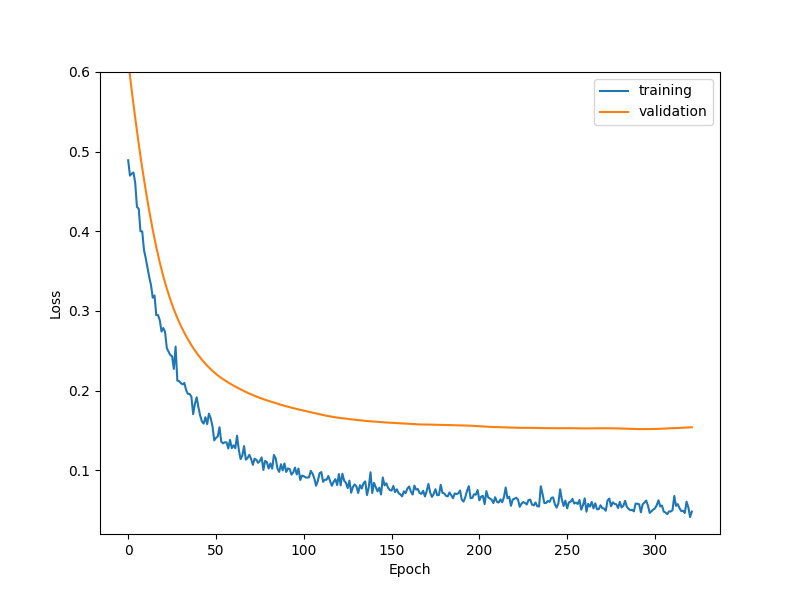
\includegraphics[height=0.48\textheight]{../project3/figures/figure3a.png}
    \column{0.5\textwidth}
    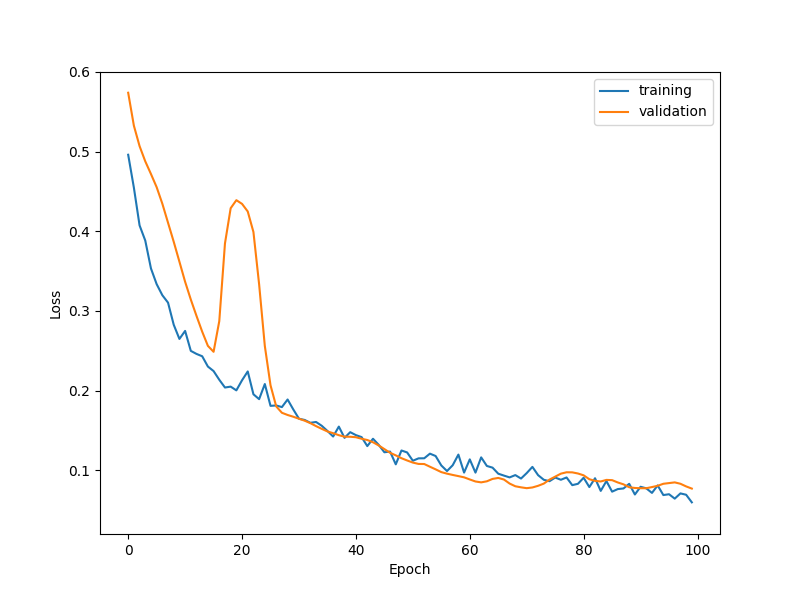
\includegraphics[height=0.48\textheight]{../project3/figures/figure3b.png}
    \end{columns}
    
    \textit{The effect of similarity between source and target on the convergence speed}
    \begin{itemize}
        \item \textit{Left: from No Lapse; right: from Static Lapse}
    \end{itemize}
    
    \note{These figures further illustrate how source-target similarity affects transfer learning performance. \\}
    \note{The left graph shows transfer from no lapse models, which has slower convergence. \\}
    \note{The right graph shows transfer from static lapse models, with faster convergence. \\}
    \note{This reinforces our finding that greater similarity between source and target domains leads to more effective knowledge transfer. \\}
\end{frame}
    

    
    \begin{frame}{Learning Curves: Transfer Knowledge to other Contract Types}
    \begin{figure}[ht]
        \centering
        \begin{subfigure}{0.48\textwidth}
            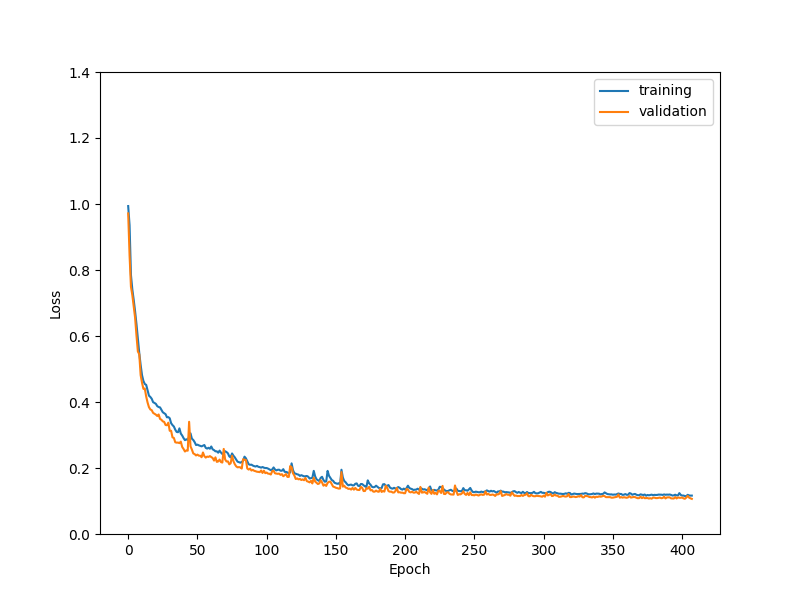
\includegraphics[width=\textwidth]{../project3/figures/figure4a.png}
            \caption{50000 samples}
        \end{subfigure}
        \begin{subfigure}{0.48\textwidth}
            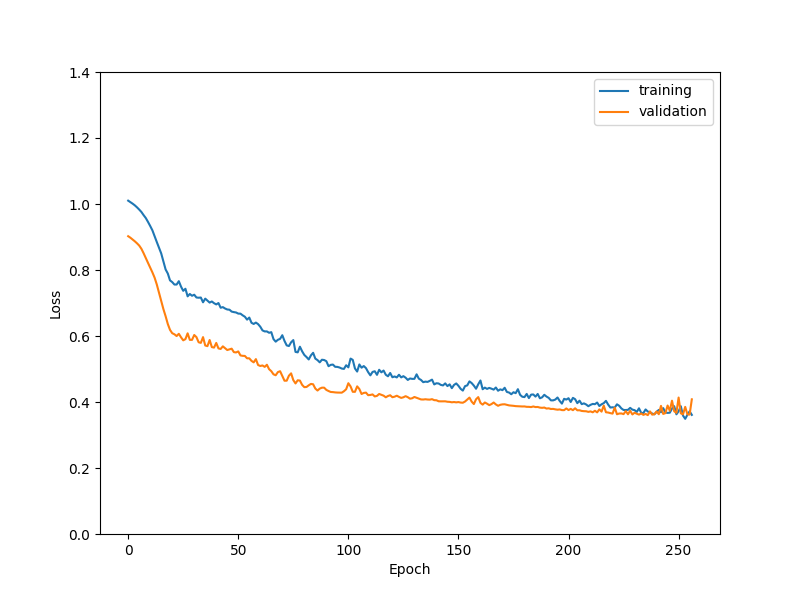
\includegraphics[width=\textwidth]{../project3/figures/figure4b.png}
            \caption{2000 samples}
        \end{subfigure}
        \caption{Learning curves of GMWB contracts}
    \end{figure}
    
    \note{These graphs show learning curves for GMWB contracts with different training sample sizes. \\}
    \note{Left figure (50,000 samples) shows that with abundant data, all methods eventually converge well. \\}
    \note{Right figure (2,000 samples) demonstrates the advantage of transfer learning in data-limited scenarios. \\}
    \note{With limited data, transfer learning methods significantly outperform training from scratch. \\}
    \note{This is particularly relevant for new products or market conditions where historical data is scarce. \\}
    \end{frame}
    
    \begin{frame}{Learning Curves: Effect of Similarity}
    \begin{figure}[ht]
        \centering
        \begin{subfigure}{0.48\textwidth}
            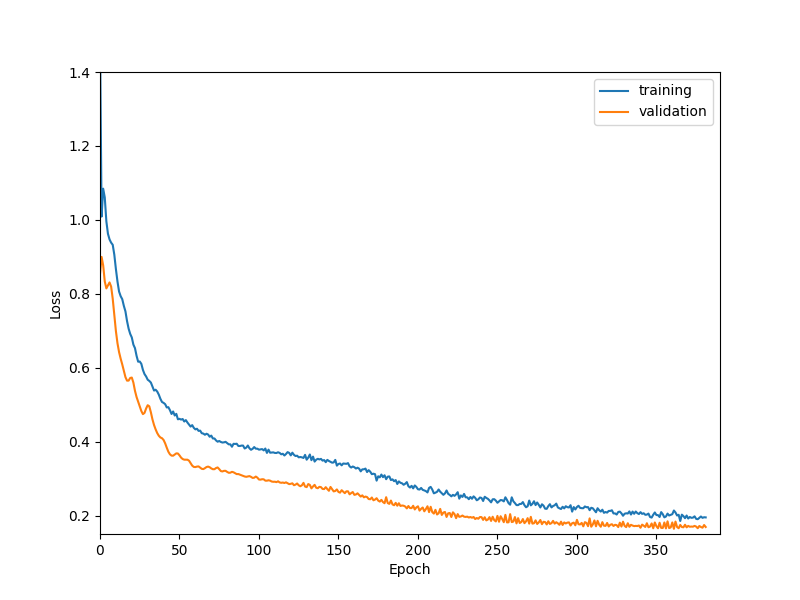
\includegraphics[width=\textwidth]{../project3/figures/figure4c.png}
            \caption{Fine-tuning}
        \end{subfigure}
        \begin{subfigure}{0.48\textwidth}
            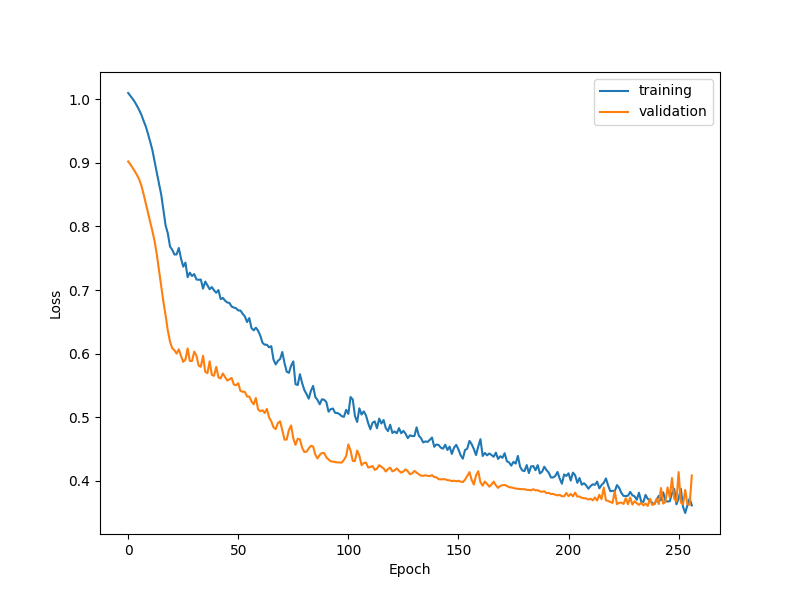
\includegraphics[width=\textwidth]{../project3/figures/figure4d.png}
            \caption{Layer Freezing}
        \end{subfigure}
        \caption{Comparison of different TL methods on GMWB contracts}
    \end{figure}
    
    
    \note{These figures compare fine-tuning vs. layer freezing approaches for GMWB contracts. \\}
    \note{Fine-tuning (left) allows all network parameters to be updated during training. \\}
    \note{Layer freezing (right) keeps early layers fixed and only updates later layers. \\}
    \note{For dissimilar contracts like GMMB to GMWB, fine-tuning generally performs better. \\}
    \note{This suggests that when transferring between different contract types, more flexibility in adaptation is beneficial. \\}
    \end{frame}
    
%     \begin{frame}{Performance Comparison (GMMB → GMWB)}
%     \begin{table}
%     \begin{tabular}{lcc}
%     \toprule
%     \textbf{Model} & \textbf{Training MSE} & \textbf{True MSE} \\
%     \midrule
%     Without TL & 0.3588 & 0.4188 \\
%     Fine Tuning & 0.1690 & 0.1780 \\
%     Layer Freezing & 0.1828 & 0.2295 \\
%     Extensive Training & 0.0853 & 0.0726 \\
%     \bottomrule
%     \end{tabular}
%     \end{table}
    
%     \begin{itemize}
%         \item Fine-tuning outperforms layer freezing for dissimilar tasks
%         \item Both TL methods better than training from scratch
%         \item Extensive training still superior with abundant data
%     \end{itemize}
    
%     \note{This table quantifies the performance of different approaches when transferring from GMMB to GMWB. \\}
%     \note{Fine-tuning (0.1780 MSE) outperforms layer freezing (0.2295 MSE) for these dissimilar contracts. \\}
%     \note{Both transfer learning methods significantly outperform training from scratch (0.4188 MSE). \\}
%     \note{With unlimited data and computational resources, extensive training (0.0726 MSE) remains the gold standard. \\}
%     \note{In practice, the trade-off between computational cost and accuracy often favors transfer learning. \\}
%     \end{frame}
    
%     \begin{frame}{Multi-task Learning}
%     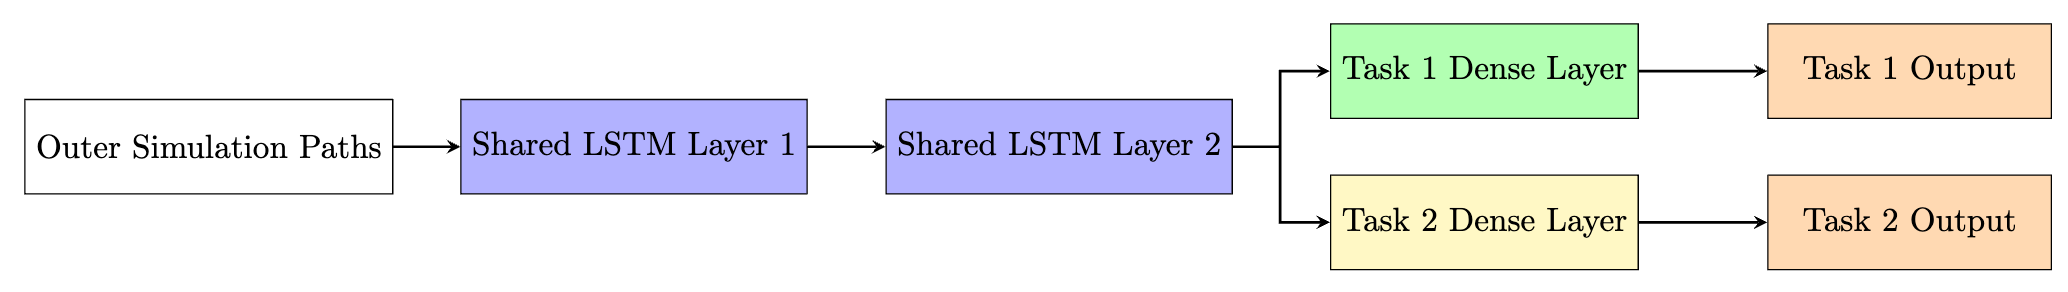
\includegraphics[width=0.9\textwidth]{../project3/figures/mtl.png}
    
%     \begin{itemize}
%         \item LSTM layers shared across multiple tasks
%         \item Task-specific fully connected layers
%         \item Objective: Minimize sum of loss functions across all tasks
%     \end{itemize}
    
%     \note{Multi-task learning offers an alternative approach to transfer learning. \\}
%     \note{Instead of sequential knowledge transfer, we train on multiple contract types simultaneously. \\}
%     \note{The shared LSTM layers capture common features across different VA contracts. \\}
%     \note{Task-specific layers then specialize for each contract type's unique characteristics. \\}
%     \note{This approach can be more efficient than training separate models for each contract type. \\}
%     \end{frame}
    
%     \begin{frame}{Multi-task Learning Framework}
%     \textbf{Input}: Set of $K$ tasks $\{\mathcal{T}_k\}_{k=1}^K$ with datasets $\mathcal{D}_k = \{(X_k^{(i)}, L_k^{(i)})\}_{i=1}^{M_k}$, shared parameters $\theta_0$, and task-specific parameters $\theta_k$ for each task $k$
      
%     \textbf{Algorithm}:
%     \begin{enumerate}
%         \item Train the multi-head LSTM metamodel on all $K$ tasks simultaneously by minimizing the multi-task loss function:
%         \begin{equation}
%             \min_{\theta_0, \{\theta_k\}_{k=1}^K} \sum_{k=1}^K \frac{1}{M_k} \sum_{i=1}^{M_k} \left( f_i(X_k^{(i)}; \theta_0, \theta_k) - L_k^{(i)} \right)^2
%         \end{equation}
%         \item Update both the shared parameters $\theta_0$ and task-specific parameters $\{\theta_k\}_{k=1}^K$ simultaneously using backpropagation and gradient descent with learning rate $\alpha$
%     \end{enumerate}
    
%     \textbf{Output}: Trained multi-task LSTM metamodel $f(\cdot; \theta_0, \{\theta_k\}_{k=1}^K)$ for all $K$ tasks
    
%     \note{This slide formalizes the multi-task learning framework mathematically. \\}
%     \note{We have $K$ different tasks (contract types) with their respective datasets. \\}
%     \note{The objective function minimizes the combined MSE across all tasks. \\}
%     \note{Parameters are divided into shared parameters $\theta_0$ and task-specific parameters $\theta_k$. \\}
%     \note{This approach encourages the model to learn generalizable features across different contract types. \\}
%     \end{frame}
    
%     \begin{frame}{Multi-task Learning: GMMB and GMWB}
%     \begin{figure}[ht]
%         \centering
%         \begin{subfigure}{0.48\textwidth}
%             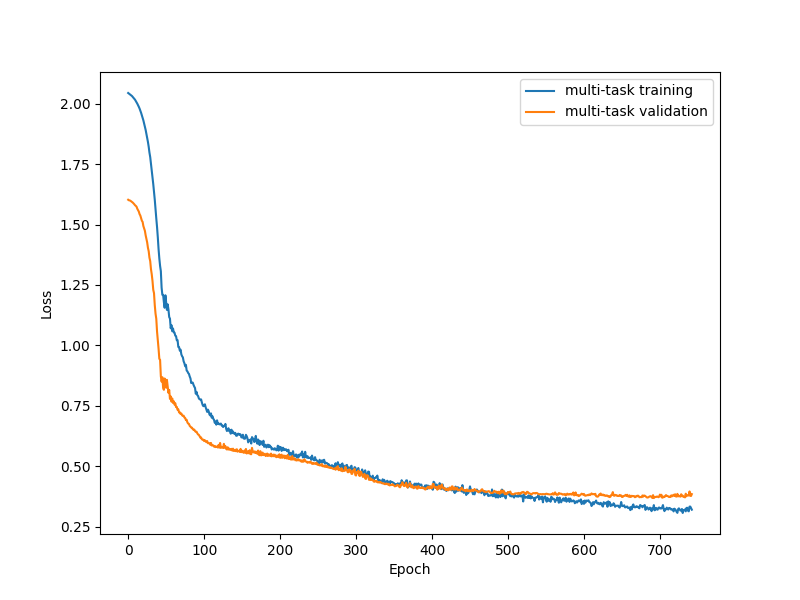
\includegraphics[width=\textwidth]{../project3/figures/figure5a.png}
%             \caption{Total MSE}
%         \end{subfigure}
%         \begin{subfigure}{0.48\textwidth}
%             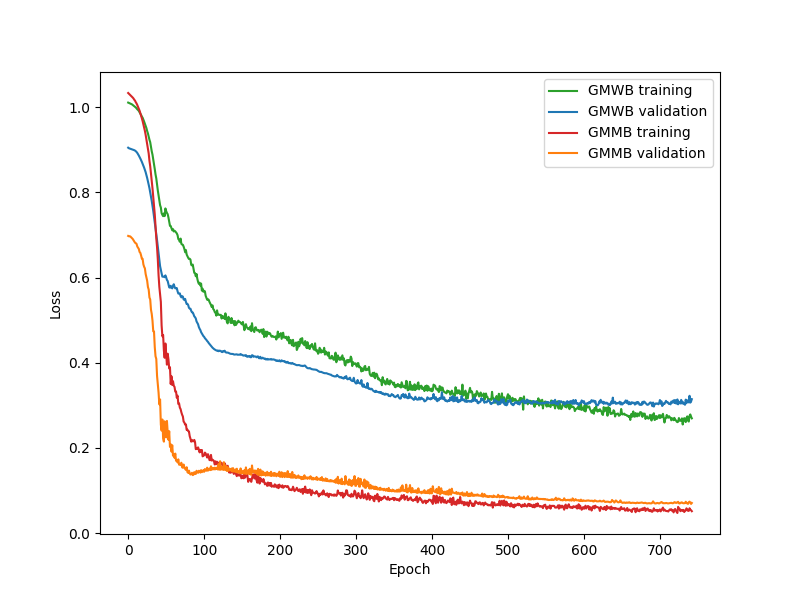
\includegraphics[width=\textwidth]{../project3/figures/figure5b.png}
%             \caption{Individual MSE}
%         \end{subfigure}
%         \caption{Multi-task learning of GMMB and GMWB}
%     \end{figure}
    
    
%     \note{These figures show the performance of multi-task learning for GMMB and GMWB contracts. \\}
%     \note{The left graph shows the total MSE across both tasks decreasing with training. \\}
%     \note{The right graph breaks down performance by individual contract type. \\}
%     \note{Multi-task learning allows knowledge sharing between contract types during training. \\}
%     \note{This can lead to better generalization, especially for the more complex contract type. \\}
%     \end{frame}
    
%     \begin{frame}{Multi-task Learning: GMMB and GMWB}
%     \begin{figure}[ht]
%         \centering
%         \begin{subfigure}{0.48\textwidth}
%             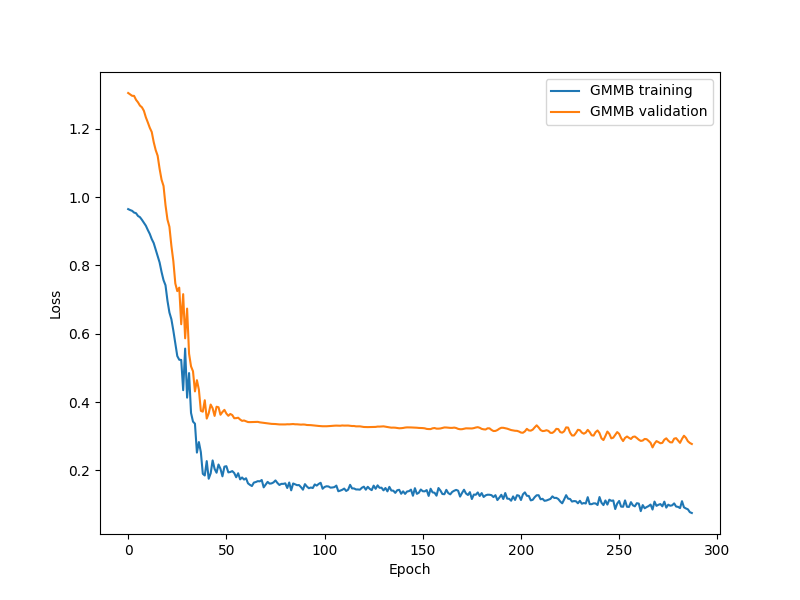
\includegraphics[width=\textwidth]{../project3/figures/figure5c.png}
%             \caption{GMMB}
%         \end{subfigure}
%         \begin{subfigure}{0.48\textwidth}
%             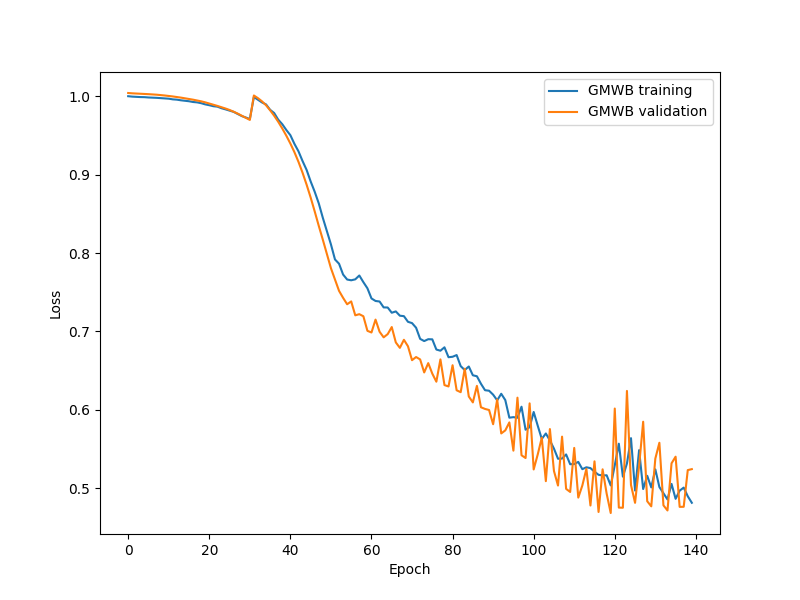
\includegraphics[width=\textwidth]{../project3/figures/figure5d.png}
%             \caption{GMWB}
%         \end{subfigure}
%         \caption{Training without multi-task learning}
%     \end{figure}
    
    
%     \note{For comparison, these figures show training curves when each contract is trained separately. \\}
%     \note{The left graph shows GMMB training alone, and the right shows GMWB training alone. \\}
%     \note{Compared to multi-task learning, individual training may converge more slowly or to higher error rates. \\}
%     \note{This demonstrates how learning multiple related tasks simultaneously can improve performance. \\}
%     \note{The shared representation forces the model to learn more robust features applicable to both contract types. \\}
%     \end{frame}
    
%     \begin{frame}{Challenges \& Limitations}
%     \begin{itemize}
%         \item Determining optimal layer freezing strategy
%         \item Handling significantly different contract structures
%         \item Quantifying uncertainty in transfer learning predictions
%         \item Regulatory acceptance of black-box approaches
%     \end{itemize}
    
%     \note{Despite promising results, several challenges remain in applying these techniques. \\}
%     \note{Finding the optimal layer freezing strategy often requires experimentation. \\}
%     \note{Very different contract structures may limit effective knowledge transfer. \\}
%     \note{Uncertainty quantification is crucial for risk management but challenging with complex models. \\}
%     \note{Regulatory concerns about model interpretability may limit practical implementation. \\}
%     \note{These challenges represent important areas for future research. \\}
%     \end{frame}
    
    \begin{frame}{Conclusions}
    \begin{itemize}
        \item Transfer learning significantly improves metamodeling for VA contracts:
        \begin{itemize}
            \item Faster training convergence
            \item Better prediction accuracy
            \item Reduced computational requirements
        \end{itemize}
        \item Enables more frequent risk assessments and faster decision-making
    \end{itemize}
    
    \note{Our research demonstrates that transfer learning significantly enhances VA contract metamodeling. \\}
    \note{The benefits include faster convergence, better accuracy with limited data, and reduced computational needs. \\}
    \note{These improvements enable more frequent and timely risk assessments. \\}
    \note{This is particularly valuable in volatile markets where rapid decision-making is essential. \\}
    \note{The approach bridges the gap between traditional actuarial methods and modern machine learning techniques. \\}
    
    \textbf{Future Work:}
    \begin{itemize}
        \item Incorporating domain knowledge into transfer process
        \item Extension to other insurance and financial products
        \item Multi-task learning with more than two tasks
    \end{itemize}
    
    \note{Several promising directions exist for extending this research. \\}
    \note{Incorporating actuarial domain knowledge could further improve transfer learning effectiveness. \\}
    \note{The approach could be extended to other insurance products and financial derivatives. \\}
    \note{Multi-task learning could be expanded to handle more than two contract types simultaneously. \\}
    \note{Integration with existing risk management systems would facilitate practical adoption. \\}
    \note{Ultimately, these techniques could transform how financial institutions manage complex product portfolios. \\}

\end{frame}



\begin{frame}
    \frametitle{References}
    \bibliographystyle{apa}
    \bibliography{../refP1, ../refP2, ../refP3}
\end{frame}
\end{document}